\DocumentMetadata{%
pdfversion=1.7,%
%pdfversion=1.3,%
xmp=false,%
testphase={new-or-1}}%
\documentclass[fleqn,s1,names,tex]{neptune}
\usepackage[5.5]{neptune-els-dtd}
%% Please do not edit bookindate/proofdate
\bookindate{2026-09-23}
\proofdate{2026-10-01}
 %% for non-CAS
 %% for CAS

\usepackage[casnptn]{neptune-els} %% for CAS


\usepackage{xcolor}
\usepackage{siunitx}


\begin{pkg}
\end{pkg}
\begin{additionalpkgs}

\end{additionalpkgs}

\usepackage{stm-els-tagpdf}
%\tagpdfsetup{paratagging-show=true}

\begin{document}
\newproof{proof}{Proof}

\long\def\stmdocshl#1{#1}
\long\def\stmdocstextcolor#1#2{#2}
\long\def\stmdocscolor#1{}

%%\def\stmdocsrangecite#1{#1} %% Add missing string in BODY and uncomment the macro

%\beginTeX\let\labelrm\rm\endTeX

%\beginXML\let\labelrm\relax\endXML

\begin{macros}
\definecolor{mgGreen}{HTML}{2CA02C} % matches SOC/SOH "Base" colour in plots
\definecolor{mgRed}{HTML}{D62728}

\def\path#1{\texttt{#1}}
\newcommand{\code}[1]{\path{#1}}
\end{macros}
\begin{additionalmacros}

\jshort
\def\xURL{URL\xspace}

\end{additionalmacros}

%%%\endheaderBC

%\CUVerifiedNoMMC
\begin{frontmatter}
%\QUERY[1]
\stmauorcid[Julia Kowal]{0000-0002-8802-6365}
\stmaucontribution[Julia Kowal]{Writing -- review \& editing,
Supervision,
Resources,
Project administration,
Funding acquisition}

\stmaucontribution[Florian Rzepka]{Writing -- review \& editing,
Writing -- original draft,
Visualization,
Validation,
Supervision,
Software,
Methodology,
Investigation,
Formal analysis,
Data curation,
Conceptualization}

\dochead{Research paper}
\title{Embedded artificial intelligence in battery management systems: Pruning and quantization for efficient state-of-charge and state-of-health estimation}

%
\addrai[1]{S0952197626026552-2a351b53fe392541ff372ee3e8955af5} 
\addrai[2]{S0952197626026552-b581eeab28175b63f74d666de5d99263} 

\begin{authorgroup}

\author{Florian Rzepka}
\cormark[1]
\cortext[1]{\COR
%\QUERY[2]
% \TFadd[\AffNum].
}
\email[florian.rzepka@tu-berlin.de]

\author{Julia Kowal}
\email[julia.kowal@tu-berlin.de]

\affiliation{o={Technical University of Berlin, Chair of Electrical Energy Storage Technology}, a={Einsteinufer 11}, c={Berlin}, p={10587}, cy={Germany}}

\end{authorgroup}

\begin{abstractgroup}
\begin{abstract}[1]
Online battery management requires accurate state-of-charge (SOC) and state-of-health (SOH) estimates within strict memory and timing budgets. To address these constraints, this work investigates how stateful long short-term memory (LSTM) networks with multi-layer perceptron (MLP) heads can be optimized for embedded artificial intelligence (AI), using structured pruning and recurrent-weight quantization to reduce memory and computational costs while retaining estimation accuracy on an STM32H753ZI microcontroller. Using the open \emph{Lithium Iron Phosphate (LFP) Cycle Ageing Dataset}, full-precision models provide the accuracy reference against which the compressed variants are evaluated. Long-horizon replay yields mean absolute error (MAE) values of 2.3--2.8 percentage points for SOC and 0.9--1.5 for SOH, showing that compression largely preserves accuracy. The evaluated 30\% pruning configuration reduces flash by 37.2\% and 43.3\% in the available firmware builds and inference time by 42.9\% and 44.0\% in the recorded hardware-in-the-loop benchmarks for SOC and SOH, respectively. The analytical complexity model relates computational savings to pruning fraction and network dimensions. Quantization reduces flash by 49.7\% and 55.9\% relative to the respective full-precision models, but raises runtime in the mixed-precision implementation. Together, the study provides a reproducible reference for resource-efficient embedded battery-state estimation.
\end{abstract}

\keywords{Embedded artificial intelligence \sep Battery state estimation \sep Long short-term memory network \sep Structured pruning \sep Weight quantization \sep Microcontroller deployment}

\end{abstractgroup}
\dataavailableat{Data availability}{The LFP DoE Cycle Ageing Dataset used in this work can be obtained from the DOI repository in~\cite{LFP_DoE_Cycle_Aging_Dataset}. The landing page provides licensing information and download instructions}
\end{frontmatter}

\begin{Nomenclature}[title=Nomenclature,labelwidth=70pt,t]
\begin{nmlist}[{Acronyms}]
\item[BMS] Battery management system
\item[SOC] State of charge
\item[SOH] State of health
\item[DoE] Design of Experiments
\item[LFP] Lithium iron phosphate
\item[LSTM] Long short-term memory network
\item[MLP] Multi-layer perceptron
\item[STM32] 32-bit ARM Cortex-M microcontroller family
\item[MAE] Mean absolute error
\item[RMSE] Root-mean-square error
\item[MAC] Multiply--accumulate operation
\item[INT8] Signed 8-bit integer representation (quantized weights)
\item[FP32] 32-bit floating-point representation
\end{nmlist}

\begin{nmlist}[Symbols]
\item[{$t$}] Time
\item[{$U(t)$}] Terminal voltage at time $t$
\item[{$I(t)$}] Current at time $t$ (positive for discharge)
\item[{$T(t)$}] Cell temperature at time $t$
\item[{$\mathrm{EFC}(t)$}] Equivalent full cycles accumulated up to $t$
\item[{$Q_c(t)$}] Cumulative charge throughput up to $t$
\item[{$C_{\mathrm{nom}}$}] Nominal discharge capacity of the cell
\item[{$C_{\mathrm{app}}$}] Apparent capacity inferred from the latest check-up
\item[{$\mathrm{DoD}$}] Depth of discharge
\item[{$\mathrm{SOC}(t)$}] State of charge at time $t$
\item[{$\mathrm{SOH}_k$}] State of health at reference cycle $k$
\item[{$\mathbf{x}_t$}] Input feature vector at time $t$
\item[{$\mathbf{h}_t$}] LSTM hidden state at time $t$
\item[{$\mathbf{c}_t$}] LSTM cell state at time $t$
\item[{$\mathbf{z}_t$}] Concatenation of input and previous hidden state at time $t$
\item[{$\mathbf{i}_t,\mathbf{f}_t,\mathbf{o}_t,\mathbf{g}_t$}] Input, forget, output, and candidate gates at time $t$
\item[{$\sigma(\cdot)$}] Logistic sigmoid activation function
\item[{$\tanh(\cdot)$}] Hyperbolic tangent activation function
\item[{$\odot$}] Element-wise (Hadamard) product
\item[{$W$}] Weight matrix (LSTM or MLP)
\item[{$b$}] Bias vector
\item[{$s$}] Per-row quantization scale (FP32)
\item[{$W^{\mathrm{fp32}},W^{\mathrm{int8}}$}] Original FP32 weight matrix and its stored INT8 representation
\item[{$\hat{W}$}] Floating-point reconstruction of an INT8 weight matrix
\item[{$\varepsilon_q$}] Positive lower bound for the quantization scale
\item[{$\mathcal{R}$}] Index set of retained LSTM hidden units
\item[{$e_n$}] Signed prediction error of sample $n$ in percentage points
\item[{$Q_p(\cdot)$}] Empirical quantile operator at probability $p$
\item[{$W_{\mathrm{ih}}^{\mathrm{int8}}$}] Quantized input-to-gate weight matrix
\nomenclbreak[labelwidth=70pt,t]
\item[{$W_{\mathrm{hh}}^{\mathrm{int8}}$}] Quantized hidden-to-gate weight matrix
\item[{$s_{\mathrm{ih}}, s_{\mathrm{hh}}$}] Per-row quantization scale vectors for $W_{\mathrm{ih}}^{\mathrm{int8}}$ and $W_{\mathrm{hh}}^{\mathrm{int8}}$
\item[{$b_{\mathrm{fp32}}$}] Floating-point bias of a given gate
\item[{$\mathbf{a}_t$}] Stacked LSTM gate pre-activation vector at time $t$
\item[{$D,H,M$}] Input dimension, LSTM hidden size, and MLP width
\item[{$N_{\mathrm{MAC}}$}] Analytical multiply--accumulate count per inference
\end{nmlist}
\end{Nomenclature}
\xalignsecondcol[-.5]
\section{Introduction}

Accurate online estimation of the state of charge (SOC) and the state of health (SOH) remains a central challenge for battery-powered systems~\citep{yaoSmarterBatteryManagement2025a,a.m.s.m.h.s.attanayakaEstimationStateCharge2019,berecibarCriticalReviewState2016,shrivastavaReviewTechnologicalAdvancement2023}. Recent reviews show sustained progress in model-based and data-driven estimators, but they also emphasize that accuracy depends strongly on cell chemistry, operating conditions, reference construction, and evaluation protocol~\citep{guoSystematicReviewElectrochemical2024,yaoSmarterBatteryManagement2025a}. For an embedded battery management system, predictive accuracy alone is therefore insufficient: the estimator must also fit the available flash and RAM, meet the update deadline, and preserve its state consistently over long input streams.

The study is motivated by modular stationary storage systems in remote microgrids. Within the MG Farm programme~\citep{leap-reMGFARMSmart,microenergyMGFARMPoweringSustainable,aqachtoulMGFARMIoTEdgeDriven2026,technischeuniversitatberlinMGFarmSmart}, partners from France, Algeria, Morocco, and Germany develop smart-grid demonstrators for North African sites. The Technical University of Berlin contributes the battery ageing experiments, the LFP DoE Cycle Ageing Dataset, a battery management system prototype, and the SOC/SOH estimators deployed on its controller. Each storage module must operate autonomously within the flash, RAM, and timing limits of an STM32H753ZI-class microcontroller. Similar constraints arise in mobile systems that cannot rely on continuous cloud access.

Existing embedded studies demonstrate that compact neural SOC or SOH estimators are feasible on microcontrollers and that quantization can reduce their storage requirements~\citep{crocioniLiIonBatteriesParameter2020,giazitzisCaseStudyTiny2024,Embedded_AI_only_SOC_mobile,Embedded_AI_SOH_badData,naguibMicroprocessorExecutionTime2022}. However, these studies generally examine one battery state, one model family, or one deployment platform. They do not provide a common, auditable comparison of structured hidden-unit pruning and recurrent-weight quantization for both stateful SOC and SOH estimators under identical long-horizon replay and hardware measurement conditions. Reproduction is further hindered when scaling parameters, recurrent-state handling, and the exact mixed-precision boundary are not reported.

This work uses the Lithium Iron Phosphate (LFP) DoE Cycle Ageing Dataset~\citep{LFP_DoE_Cycle_Aging_Dataset}. It contains long-term cyclic ageing measurements from multiple LFP cells under full and fractional factorial conditions, with controlled temperature, charge and discharge rates, depth-of-discharge variations, and interleaved capacity, open-circuit-voltage, and pulse-power check-ups. These data support a paired assessment of rapid SOC dynamics and slowly evolving SOH trajectories.\beginTeX\eject \mbox{}\\ \mbox{}\\ \endTeX

The objective of this study is to quantify, under identical data and deployment conditions, how structured hidden-unit pruning and recurrent-weight post-training quantization change the accuracy, memory footprint, and inference cost of stateful LSTM\,+\,MLP SOC and SOH estimators on an STM32H753ZI. The study makes three contributions:
\begin{enumerate}[label=(\roman*),leftmargin=*,nosep]
\item an auditable path from trained PyTorch models to stateful C inference, including explicit feature scaling, recurrent-state handling, pruning, and mixed-precision quantization.
\item a controlled Base--Pruned--Quantized comparison for both SOC and SOH using continuous replay, linked-firmware flash and RAM, host latency, and cycle-counter-measured kernel time.
\item an evidence-bounded trade-off analysis that connects  \ubrk  architecture-level operation counts and implementation details to long-horizon accuracy, filtering, and application-dependent utility.
\end{enumerate}
The novelty lies in this paired, transparent deployment and compression benchmark rather than in proposing a new recurrent cell or compression algorithm.

\section{Related Work and Motivation}

\subsection{{\?{SOC}}/\?{SOH} Estimation}

Existing SOC/SOH estimation methods can be grouped into three families~\citep{a.m.s.m.h.s.attanayakaEstimationStateCharge2019,berecibarCriticalReviewState2016,shrivastavaReviewTechnologicalAdvancement2023,guoSystematicReviewElectrochemical2024}. First, \emph{measurement-derived} techniques use Coulomb counting and open-circuit-voltage (OCV) look-up tables during rest periods. They provide inexpensive proxies but suffer from drift, offset accumulation, and a strong dependence on initialization and periodic recalibration. Second, \emph{model-based} observers combine equivalent-circuit or electrochemical models with Kalman filtering and its variants. These approaches can offer physical interpretability but require careful parameter identification and are sensitive to model mismatch and ageing-induced parameter drift. Third, \emph{data-driven} methods employ machine-learning regressors, including LSTM networks, Transformers, and hybrid structures, to map sequences of current, voltage, and temperature to SOC and SOH estimates. Key challenges for such models are robustness when operated under conditions that differ from the training data and the careful treatment of normalization and state handling on embedded targets.

Recent hybrid estimators combine physical or statistical preprocessing with learned correction models. \citet{wang_improved_2024} couple online parameter identification with an adaptive radial-basis correction and differential support-vector machine for SOC estimation under dynamic vehicle-oriented tests. For whole-life capacity estimation, \citet{wang_improved_2023} combine singular filtering, Gaussian-process regression, and an LSTM to address fast ageing and varying currents. These studies broaden the operating conditions and model structures considered for battery-state estimation. Their primary evidence concerns estimation accuracy, however. Neither reports a paired post-training pruning and quantization study with linked-firmware memory and recurrent microcontroller timing. They are therefore complementary to, rather than substitutes for, the deployment benchmark developed here.
Across these families the reported accuracy spans a wide range. Electrochemical or Equivalent Circuit Model (ECM)-based observers with carefully tuned filters often achieve SOC root-mean-square errors (RMSE) well below 1\% of full scale and sub-percent SOH capacity errors on laboratory test cycles~\citep{gaoCoEstimationStateofChargeStateof2022,gaoEnhancedStateofchargeEstimation2022,shenAlternativeCombinedCoestimation2022,wangFusionEstimationLithiumion2022}. Recent sequence-model approaches based on N-BEATS and Bidirectional LSTMs (BiLSTMs) for sodium-ion cells report SOC Mean Absolute Error (MAE) between roughly 0.1 and 0.4\%~\citep{sunStateChargeEstimation2023,sunStateofchargeEstimationSodiumion2024}, whereas TinyML-style SOC estimators deployed on microcontrollers often operate in the 1--3\% error regime~\citep{crocioniLiIonBatteriesParameter2020,giazitzisCaseStudyTiny2024,Embedded_AI_only_SOC_mobile}. These values provide context rather than a direct ranking because chemistry, data splits, target construction, drive cycles, and error definitions differ between studies.
Kalman filters, particle filters, and equivalent-circuit-model observers therefore dominate the classical literature, yet their accuracy can degrade over long operating periods with pronounced current and temperature gradients~\citep{gaoEnhancedStateofchargeEstimation2022,wangFusionEstimationLithiumion2022}. Recurrent neural networks, and in particular LSTM-based regressors, address these limitations by integrating long temporal context and absorbing residual modelling errors~\citep{liOnlineCapacityEstimation2021,wangFusionEstimationLithiumion2022}. In this work we deliberately restrict the architecture search to a single-layer LSTM with a fully connected Multi-Layer Perceptron (MLP) output layer. LSTMs retain explicit cell states with separate input, forget, and output gates, which made it straightforward to hand-code a numerically stable, stateful kernel in C and to reuse the same backbone for both SOC and SOH. Gated recurrent units (GRUs) or Transformer variants could offer alternative trade-offs between accuracy and cost, but exploring multiple architectures would dilute the focus on the embedded tool flow and is left as future work.
Most publications on LSTM-based estimators maximize accuracy with complex architectures and rarely examine how the resulting models behave once deployed on constrained controllers. Even within the LSTM family, sliding-window inference is commonly employed because it delivers high accuracy, but it also requires substantial RAM to buffer multiple past samples. A stateful LSTM that hands over its hidden and cell vectors step by step retains the temporal information without maintaining large windows and therefore forms the first optimization step in our architecture. The associated handling of hidden states, feature scaling, and numerical stability is rarely described in the literature, which is why this work explicitly targets embedded SOC/SOH deployment (see \xref{TeXFolio:fig1}).
%\QUERY[3]
\begin{figure*}
\caption{\xlabel{fig:lstm_mlp_schematic}Schematic of the deployed SOC/SOH estimator. Preprocessed feature streams are fed into a single-layer LSTM whose hidden state is propagated across time. At each step a lightweight MLP head maps the hidden representation either to SOC or SOH, enabling stateful streaming inference on the STM32.}
\includegraphics{gr1}
\end{figure*}

\subsection{Embedded Deployment Strategies}

Commercial toolchains such as ONNX Runtime, TensorRT, and STM32Cube.AI support many neural-network deployment workflows   \ubrk \citep{ONNXRuntimeHighperformance,NVIDIATensorRTHighPerformance,XCUBEAISTM32CubeExpansion}. For continuously stateful estimators, however, a generated binary does not always expose recurrent-state handling or the precise placement of mixed-precision scaling operations needed for an implementation audit. \citet{naguibMicroprocessorExecutionTime2022} compare accuracy, execution time, flash, and RAM for classical and neural SOC estimators on two NXP microcontrollers. \citet{crocioniLiIonBatteriesParameter2020} deploy compact recurrent capacity estimators on STM32 targets and study 8-bit quantization. More recent TinyML studies evaluate quantized or hardware-accelerated SOC estimators on embedded platforms~\citep{giazitzisCaseStudyTiny2024,Embedded_AI_only_SOC_mobile}, while \citet{Embedded_AI_SOH_badData} target computationally compact SOH estimation. These studies establish embedded feasibility, but each addresses a narrower combination of task, architecture, compression method, and target hardware.

At the compression-method level, PQ Bench~\citep{schulzePQBenchBenchmarking2025} systematically compares pruning and quantization across general deep-learning workloads and confirms that their accuracy--storage trade-offs are model dependent. It does not address the continuous recurrent state, SOH post-processing, or microcontroller timing behaviour of battery estimators. The resulting research gap is therefore not the absence of compact neural estimators, but the absence of a controlled, task-paired benchmark that traces two transparent compression routes from trained SOC and SOH models to measured stateful firmware behaviour. Our study addresses this gap with the same input dimension, streaming protocol, performance-indicator definitions, and STM32 measurement procedure for Base, Pruned, and Quantized variants of both tasks.

To retain control over the implementation boundary, we extract the PyTorch tensors, remove complete recurrent channels according to the documented saliency score, apply per-row symmetric quantization to the recurrent weights, and implement the LSTM gates and activations in C. This path makes the state update, scaling operations, and stored parameter types inspectable and links the model transformations directly to the reported flash, RAM, and timing measurements.

\section{Dataset and Preprocessing}

\subsection{Ageing Experiments and Load Profiles}

All experiments rely on the high-resolution LFP DoE Cycle Ageing Dataset~\citep{LFP_DoE_Cycle_Aging_Dataset}. The measurements originate from a design-of-experiments study on commercially available JGCFR18650-1800mAh-3.2V LFP cells~\citep{jgneJGCFR186501800mAh32VProductSpecification} conducted at the Technical University of Berlin. Cells were cycled inside a climatic chamber at 25~{\degree}C while the following factors were systematically varied:
\begin{align}
C_{\mathrm{chg}} &\in [0.5\,\mathrm{C},\,0.9\,\mathrm{C}],\\
C_{\mathrm{dis}} &\in [1.0\,\mathrm{C},\,2.5\,\mathrm{C}],\\
\mathrm{DoD} &\in [45\%,\,65\%].
\end{align}
The mixed full/fractional factorial plan distributes fifteen test cells across eight operating-point combinations and includes replication to assess repeatability.  \xref{fig:doe_cube} shows the low and high levels of all three factors.

Between ageing loops, dedicated check-ups provide capacity tests, open-circuit-voltage sweeps, and hybrid pulse-power characterization. Stationary-storage profiles are additionally injected to emulate realistic power flows~\citep{kucevicStandardBatteryEnergy2020a}. These profiles originate from residential photovoltaic home-storage applications and contain stochastic load and generation patterns that excite the cell differently from constant-current cycling.

The raw dataset contains uniformly sampled measurements at \SI{1}{\hertz}, including voltage, current, terminal temperature, and auxiliary channels. Partitioned Parquet tables support efficient retrieval of the long ageing sequences.
The dataset is published in \citet{LFP_DoE_Cycle_Aging_Dataset}. The cube notation follows standard DoE conventions as summarized in \citet{siebertzStatistischeVersuchsplanung2017}.
Together,  \xref{fig:soc_tests,fig:soh_all_days} illustrate the diversity of SOC transients and ageing behaviour that the estimators must capture: short-term SOC dynamics are driven by fast current swings and mode changes between profiles, whereas SOH evolves slowly over hundreds of days and depends on the cumulative operating conditions of each cell.

\begin{figure}
\caption{\xlabel{fig:doe_cube}General three-factor design-of-experiments geometry used to structure the LFP ageing campaign. The cube represents the factorial design space, while the generic labels $y_1$ to $y_{15}$ denote experimental conditions within and around it. The dataset-specific charge rate, discharge rate, and depth-of-discharge levels are described in the accompanying text.}
\includegraphics[width=\columnwidth]{gr2}
\end{figure}

\begin{figure}
\caption{\xlabel{fig:soc_tests}Representative SOC trajectory illustrating selected segments of the experimental protocol used in this study. The plot shows a portion of the cyclic ageing procedure with defined charge and discharge currents and a specified depth-of-discharge (DoD), followed by the diagnostic checkup sequence comprising OCV determination, HPPC pulses, and capacity tests. In addition, the trajectory includes a load profile taken from a stationary battery storage system. Together, these segments capture both controlled laboratory diagnostics and application-oriented operating conditions.}
\includegraphics[width=\columnwidth]{gr3}
\end{figure}

\begin{figure}
\caption{\xlabel{fig:soh_all_days}Evolution of the state of health across all LFP cells in the ageing campaign, shown over the total experimental duration. The spread between trajectories reflects the different operating points in the factorial plan (C-rates, depth of discharge, profile mix) and motivates the use of a data-driven SOH estimator that generalizes across cells and loading conditions.}
\includegraphics[width=\columnwidth]{gr4}
\end{figure}

\subsection{Feature Engineering}

The SOC model consumes the six-dimensional feature vector
\begin{equation}
\mathbf{x}^{\mathrm{SOC}}_t = \bigl[U(t),\, I(t),\, T(t),\, Q_c(t),\, \tfrac{\mathrm{d}U}{\mathrm{d}t}(t),\, \tfrac{\mathrm{d}I}{\mathrm{d}t}(t)\bigr],
\end{equation}
where the audited preprocessing uses timestamp-aware backward differences rather than centred differences. For sample index $k>0$,
\begin{align}
\Delta t_k &= \max(t_k-t_{k-1},\varepsilon_t), \qquad \varepsilon_t=10^{-6},\xlabel{eq:feature_dt}\\
\left.\frac{\mathrm{d}U}{\mathrm{d}t}\rf\vert_k &= \frac{U_k-U_{k-1}}{\Delta t_k}, \qquad
\left.\frac{\mathrm{d}I}{\mathrm{d}t}\rf\vert_k = \frac{I_k-I_{k-1}}{\Delta t_k}.\xlabel{eq:feature_backward_difference}
\end{align}
This causal calculation requires only the preceding voltage/current sample and timestamp and has constant work per update. In the evaluated benchmark, however, derivative and cumulative channels were prepared host-side before replay. Complete six-feature vectors were transmitted via UART, and the firmware applied the same robust-scaling parameters used during model development. Consequently, the reported DWT kernel times exclude sensor acquisition and feature construction. The exact placement of the six-feature scaling operation is documented with the STM32 measurement interval below. Each component is normalized using a robust scaling operation based on the median $m$ and interquartile range $r$:
\begin{equation}
\tilde{x}^{\mathrm{SOC}}_{t,k} = \frac{x^{\mathrm{SOC}}_{t,k} - m_k}{r_k + \varepsilon}, \qquad \varepsilon=10^{-6}.
\end{equation}
The same $(m_k,r_k)$ pairs are embedded in the firmware so that host and STM32 inputs are normalized identically.
The SOH model uses a slightly different feature stack to capture slow-varying degradation markers:
\begin{equation}
\mathbf{x}^{\mathrm{SOH}}_t = \bigl[t,\, U(t),\, I(t),\, T(t),\, \mathrm{EFC}(t),\, Q_c(t) \bigr],
\end{equation}
where $t$ is the cumulative time stamp and $\mathrm{EFC}(t)$ denotes the equivalent full cycles accrued up to sample $t$. These channels are likewise robustly normalized, relying on median and interquartile range rather than mean and variance to reduce the influence of outliers in current and voltage measurements~\citep{huberRobustStatistics2009,pedregosaScikitlearnMachineLearning2012}. During deployment, the SOC and SOH models run independently on the microcontroller and each\xvadjust[\xpagebreak] produces one estimate per second. In principle, both estimates could be fused more tightly, but this work keeps the models separate to evaluate their resource use and accuracy independently.

\subsection{Reference {\?{SOC}} and {\?{SOH}} targets}

The ground-truth SOC trajectory is derived from Coulomb counting with drift compensation. Denoting the apparent cell capacity after a given check-up by $C_{\mathrm{app}}$, the SOC inside a charge--discharge segment is computed as
\begin{equation}
\mathrm{SOC}(t) = \mathrm{SOC}(t_0) - \frac{1}{C_{\mathrm{app}}}\int_{t_0}^{t} I(\tau)\,\mathrm{d}\tau,
\end{equation}
where the integral is reset to $\mathrm{SOC}=1$ after each constant-voltage (CV) termination. The reset mitigates the bias that would otherwise accumulate due to capacity fade, yet the long-term traces still reveal gradual changes in the SOC envelope as $C_{\mathrm{app}}$ decreases.
State of health is obtained from the periodic capacity check-ups through
\begin{equation}
\mathrm{SOH}_k = \frac{C_k}{C_{\mathrm{nom}}},
\end{equation}
with $C_k$ representing the measured discharge capacity during the $k$th reference cycle (comprising capacity test, open-circuit-voltage sweep, and hybrid pulse-power characterization) relative to the nominal capacity $C_{\mathrm{nom}}$. These targets highlight the need for a data-driven estimator that remains accurate despite the evolving capacity landscape, which motivates the use of recurrent neural networks for both SOC and SOH predictions.
The reference SOC and SOH traces are therefore offline constructs. They rely on information that is not available in deployment, such as long rest periods for OCV stabilization and capacity from periodic full cycles, and they assume perfect initialization and recalibration. These constructions follow common practice in battery management, where SOC is obtained by Coulomb counting and SOH is expressed as the ratio between present and nominal capacity~\citep{plettBatteryManagementSystems2015,a.m.s.m.h.s.attanayakaEstimationStateCharge2019,berecibarCriticalReviewState2016}. On the STM32 the estimators operate purely on the streamed measurements and their internal states. The reference trajectories only serve as ground truth for training and evaluation.

\subsection{Streaming inference setup}

Because the SOC and SOH estimators are stateful, the LSTM hidden and cell states are continuously forwarded from one sample to the next along the full input stream. At each sampling instant the current feature vector is processed together with the previous hidden and cell states, which yields the new states and the corresponding SOC or SOH estimate. We therefore operate the models in a purely step-by-step streaming regime without forming sliding input windows. On the host the full normalized sequence from the LFP DoE Cycle Ageing Dataset is processed once in this fashion, and the resulting SOC and SOH estimates are aligned with the reference trajectories. On the STM32 firmware the same step-wise LSTM implementation is used, driven by the UART feature stream, so that host and embedded benchmarks reflect identical inference conditions. The streaming dashboards in  \xref{fig:soc_dashboard,fig:soh_dashboard} illustrate a complete run for one representative cell.

\subsection{{\?{SOH}} prediction post-processing}\xlabel{sec:soh_filter_method}
The SOH trajectories in the final dashboard use two sequential causal filtering stages. First, each raw model output $\hat y_t$ is multiplicatively aligned with the initial SOH label, $\hat y_t^{(0)}=(y_0/\hat y_0)\hat y_t$. Stage~1 limits the change of this calibrated prediction relative to the preceding stage output to
\begin{equation}
\ell_t = \min\!\left(10^{-4}\lvert y_{t-1}^{(1)}\rvert,10^{-5}\right),
\end{equation}
and subsequently applies an exponential moving average (EMA) with $\alpha_1=0.02$. The limiter is symmetric, so positive and negative proposal changes are both restricted to $\pm\ell_t$. Stage~2 consumes the complete stage-1 trajectory, applies another EMA with $\alpha_2=10^{-6}$, and limits only downward changes according to
\begin{equation}
y_t^{(2)}={\max}\!\left(e_t^{(2)},y_{t-1}^{(2)}-2\times10^{-8}\right),\qquad
e_t^{(2)}=(1-\alpha_2)e_{t-1}^{(2)}+\alpha_2 y_t^{(1)}.
\end{equation}
Thus, the curve in  \xref{fig:soh_dashboard} is not obtained by applying $\alpha_2$ directly to an unfiltered network output.

For an EMA sampled at interval $\Delta t$, the equivalent time constant and cutoff frequency are
\begin{equation}
\tau=-\frac{\Delta t}{\ln(1-\alpha)},\qquad
f_{\mathrm c}=\frac{1}{2\pi\tau}.
\end{equation}
At the dataset rate of \SI{1}{\hertz}, stage~1 has $\tau=\SI{49.5}{\second}$, $f_{\mathrm c}=\SI{3.22}{\milli\hertz}$, and an EMA-only 90\% step-response time of approximately \SI{114}{\second}. For stage~2, $\tau$ is approximately 11.57~days, $f_{\mathrm c}=1.59\times10^{-7}$~Hz, and the corresponding 90\% time is 26.65~days. These frequencies characterize only the linear EMA components. The nonlinear rate limiters have no single cutoff frequency. The very strong second stage can reduce error against slowly varying labels while introducing substantial response delay, which is evaluated separately in~\xref{app:soh_filter}.

\section{Model Architecture and Baseline Performance}

\subsection{{\?{LSTM}} architecture in \?{PyTorch}}

Both SOC and SOH estimators employ the same recurrent equation set but differ in size according to their training releases. The SOC configuration uses $H=64$ hidden units and an MLP output layer of width~64, whereas the SOH configuration increases both dimensions to~128 to cope with the longer temporal context. LSTM gates $i_t,f_t,o_t$ and candidate state $g_t$ follow the standard formulation used in modern RNN surveys~\citep{liptonCriticalReviewRecurrent2015}. All models are implemented in PyTorch~\citep{paszkePyTorchImperativeStyle2019}.
For one streaming update with input dimension $D=6$, LSTM hidden size $H$, and fixed MLP width $M$, the matrix products require
\begin{equation}
N_{\mathrm{MAC}}(H)=4H(D+H)+HM+M,
\xlabel{eq:model_macs}
\end{equation}
where one multiply--accumulate (MAC) is counted per weight. Bias additions, nonlinearities, indexing, and memory transfers are excluded. For a hidden-unit pruning fraction $p$, the retained hidden size is $H_p=(1-p)H$. Substitution into Eq.~\neqref{eq:model_macs} gives the relative analytical MAC reduction
\begin{align*}
R_{\mathrm{MAC}}(H,p)
&=1-\frac{N_{\mathrm{MAC}}((1-p)H)}{N_{\mathrm{MAC}}(H)}\\
&=\frac{4(2p-p^2)H^2+p(4D+M)H}
{4H^2+(4D+M)H+M},\\
\lim_{H\rightarrow\infty}R_{\mathrm{MAC}}(H,p)&=2p-p^2.
\end{align*}
The quadratic recurrent term is therefore reduced by $2p-p^2$, the linear input and MLP terms by $p$, and the fixed output term is unchanged. The finite-model reduction is a weighted combination of these contributions and remains below the large-$H$ limit. For the evaluated fraction $p=0.30$, this limit is 51\%. The implemented integer dimensions give 22,080 to 12,124 MACs for SOC ($64\rightarrow45$), a 45.1\% reduction, and 85,120 to 46,208 MACs for SOH ($128\rightarrow90$), a 45.7\% reduction. \xref{app:model_complexity} visualizes both this operating point and the general dependence on $p$. The relation makes the computational effect of a selected hidden-size reduction predictable before deployment, while hardware measurements translate the analytical reduction into platform-specific flash, latency, and energy changes.
\begin{align}
\mathbf{z}_t &= [\mathbf{x}_t,\mathbf{h}_{t-1}],\\
\mathbf{i}_t &= \sigma(W_i \mathbf{z}_t + \mathbf{b}_i), \quad
\mathbf{f}_t = \sigma(W_f \mathbf{z}_t + \mathbf{b}_f), \nonumber\\
\mathbf{o}_t &= \sigma(W_o \mathbf{z}_t + \mathbf{b}_o), \quad
\mathbf{g}_t = \tanh(W_g \mathbf{z}_t + \mathbf{b}_g), \nonumber\\
\mathbf{c}_t &= \mathbf{f}_t \odot \mathbf{c}_{t-1} + \mathbf{i}_t \odot \mathbf{g}_t,\quad
\mathbf{h}_t = \mathbf{o}_t \odot \tanh(\mathbf{c}_t). \nonumber
\end{align}
Eqs.~\neqref{eq:model_macs} and the recurrent update above define the common Base architecture used for both tasks. Pruning changes its hidden dimension and parameter submatrices, whereas quantization changes the stored representation of selected recurrent weights. Neither transformation changes the input features, targets, or streaming state-update order.

Both SOC and SOH models are trained with a mean-squared-error loss between the prediction and the corresponding reference at each training sample. During validation we additionally report mean absolute error (MAE), root-mean-square error (RMSE), and $R^2$. The trained parameters, configuration files, and optimizer statistics are retained to enable deterministic replay of both models.

\subsection{Training Notes}

Training is carried out on a GPU node equipped with NVIDIA A100-class accelerators using mixed-precision (FP16) arithmetic. Both models use the AdamW optimiser with cosine-annealing warm-restart scheduling, gradient clipping, and mini-batch training~\citep{loshchilovDecoupledWeightDecay2017,loshchilovSGDRStochasticGradient2016,micikeviciusMixedPrecisionTraining2017,pascanuDifficultyTrainingRecurrent2012}. The SOC configuration uses a learning rate of $1.5\times10^{-4}$, a batch size of~512, and sequence chunks of length~2024. The corresponding SOH values are $2.0\times10^{-4}$, 128, and 2048.

Deployment operates the LSTM in stateful, step-by-step streaming mode, whereas training uses truncated backpropagation through time over these chunks. Hidden and cell states are propagated within every chunk in the same temporal order as during deployment. Chunking permits randomized segment sampling and tractable gradient computation without changing the recurrent update equations.

\subsection{Baseline Accuracy}

On the workstation the SOC and SOH base models are first evaluated in streaming mode on the full ageing trajectory of one representative LFP cell from the LFP DoE Cycle Ageing Dataset~\citep{LFP_DoE_Cycle_Aging_Dataset}, yielding baseline MAE and RMSE values for both tasks. These Python replays operate on the original PyTorch implementations and provide the numerical reference for the compression experiments. The corresponding trained models are pruned, quantized, and exported to STM32 firmware, where identical feature streams are replayed to measure accuracy, flash and RAM usage, system latency, and on-device inference time. A timing-derived energy proxy is calculated as described in  \xref{sec:kpis}.  \xref{fig:pipeline} summarizes this training-to-firmware benchmarking pipeline.

\begin{figure*}
\caption{\xlabel{fig:pipeline}End-to-end pipeline from dataset to embedded benchmarking. The LFP DoE Cycle Ageing Dataset feeds PyTorch training on a GPU workstation. The resulting SOC and SOH LSTM\,+\,MLP models are pruned and quantized, exported as C headers, and deployed on an STM32H753ZI board, where flash/RAM usage, inference time, and latency are measured under streaming replay. Estimated energy per inference is derived from kernel time under a constant board-power assumption.}
\includegraphics{gr5}
\end{figure*}

\section{Pruning}

Pruning reduces the size and computational cost of a neural network by eliminating parameters or whole units that contribute little to the overall mapping, while keeping the input--output behaviour as close as possible to the dense baseline~\citep{hanLearningBothWeights2015,blalockWhatStateNeural2020}. In our setting we apply structured pruning at the level of complete LSTM hidden units so that the resulting model remains well suited for efficient C implementations on the microcontroller.

\subsection{Structured magnitude pruning}

Structured magnitude pruning removes the lowest-saliency LSTM units until only 45 hidden channels remain in the SOC model (30\% sparsity), with analogous settings for the SOH experiments. Reducing the state dimension is a prerequisite for fitting the estimators into the flash and SRAM budgets of the target STM32-based BMS and for shortening the on-device inference time, inspired by structured sparsity approaches for deep and recurrent networks~\citep{wenLearningStructuredSparsity2016,lobachevaStructuredSparsificationGated2020,narangExploringSparsityRecurrent2017}. In analogy to the group-lasso style regularizers proposed for LSTMs in \citet{wenLearningStructuredSparsity2016,lobachevaStructuredSparsificationGated2020}, which aggregate weights across gates via L2 norms, we define a saliency score for each hidden unit $h$ that combines all incoming weights from the different gates:
\begin{equation}
\xlabel{eq:pruning_saliency}
s_h = \sum_{g\in\{i,f,o,g\}} \left(\lVert W_{\mathrm{ih}}^{(g)}[h,:]\rVert_2 + \lVert W_{\mathrm{hh}}^{(g)}[h,:]\rVert_2\right).
\end{equation}
Units are ranked by $s_h$, and the $H'$ highest-scoring indices form the retained set $\mathcal{R}$. For each gate $g$, structured pruning constructs the reduced matrices
\begin{align}
\widetilde{W}_{\mathrm{ih}}^{(g)} &= W_{\mathrm{ih}}^{(g)}[\mathcal{R},:],\nonumber\\
\widetilde{W}_{\mathrm{hh}}^{(g)} &= W_{\mathrm{hh}}^{(g)}[\mathcal{R},\mathcal{R}],\nonumber\\
\widetilde{W}_{\mathrm{MLP},1} &= W_{\mathrm{MLP},1}[:,\mathcal{R}].
\xlabel{eq:pruning_slicing}
\end{align}
Thus the same index set removes gate rows, recurrent columns, and the corresponding inputs of the first MLP layer. The reduced tensors remain dense. The computational saving comes from the smaller dimension rather than sparse indexing.

The final SOC deployment uses $H'=45$ instead of 64 hidden units, while SOH uses $H'=90$ instead of 128. Both transformations remove approximately 30\% of the recurrent channels. The fraction $p=0.30$ was selected as a single moderate operating point that provides a substantial dimensional reduction while retaining useful estimator accuracy. It was not obtained from an exhaustive pruning-rate sweep and is not claimed to be optimal. Establishing an optimal fraction would require separately pruned and fine-tuned models for each candidate rate and is reserved for a pruning-focused investigation. This is a one-shot structured operation followed by brief post-pruning fine-tuning. No iterative pruning schedule or pruning-aware training is used. The L2 aggregation gives a gate-consistent ranking that can be calculated directly from the model weights and mapped to dense C arrays. \xref{app:pruning_diagnostics} reports the resulting SOC saliency ranking and recurrent-weight distributions. These diagnostics describe the resulting weight selection but do not establish a causal regularization effect.
The criterion is selected because it combines all four gate rows for one recurrent unit and maps directly to removal of dense rows, recurrent columns, and the associated MLP input. It therefore provides a reproducible, gate-consistent ranking that translates directly into a smaller dense kernel. Gradient sensitivity would additionally use training data and backpropagation, while activation-based ranking would use a representative calibration stream and a temporal aggregation rule. A future comparison with these data-dependent alternatives can determine whether their additional information further improves the accuracy--efficiency trade-off. \xref{app:pruning_criterion_scope} summarizes the method properties (see \xref{TeXFolio:fig6,TeXFolio:fig7}).

\begin{figure}
\caption{\xlabel{fig:pruning_schematic}Structured hidden-channel pruning used in this study. Panel (a) marks one low-saliency LSTM channel and its incident connections in red. Panel (b) shows the resulting dense network after removing the corresponding gate rows, recurrent columns, and MLP input column according to Eq.~\neqref{eq:pruning_slicing}. The final SOC and SOH hidden dimensions are shown between the panels.}
\includegraphics[width=\columnwidth]{gr6}
\end{figure}

\begin{figure*}
\caption{\xlabel{fig:quantization_schematic}FP32-to-INT8 quantization and embedded deployment. The recurrent FP32 weight matrices are mapped row by row to signed INT8 codes in the symmetric set $\{-127,\ldots,127\}$ together with one FP32 scale per row. The integer recurrent weights and scale vectors are exported as C headers and combined with FP32 biases, activations, recurrent states, and MLP operations in the STM32 kernel.}
\includegraphics{gr7}
\end{figure*}

\subsection{Resulting pruned models}

The resulting pruned SOC and SOH models still run in FP32 but reduce flash consumption and runtime considerably once compiled for STM32.  \xref{sec:kpis} summarizes the corresponding latency and memory savings. These pruned variants are evaluated alongside their base and quantized counterparts throughout the results section.

\section{Quantization}

Quantization complements pruning by reducing the numerical precision of selected weights while keeping the network topology unchanged. We apply post-training, weight-only quantization to the LSTM input-to-hidden matrix $W_{\mathrm{ih}}$ and hidden-to-hidden matrix $W_{\mathrm{hh}}$. The resulting matrices are stored as 8-bit integers together with one FP32 scale per row. Biases, activations, recurrent hidden and cell states, and the MLP remain FP32. This design concentrates the storage reduction on the dominant recurrent matrices while retaining a mixed-precision computation path.

\subsection{Per-row symmetric quantization}

The FP32 matrices $W_{\mathrm{ih}}^{\mathrm{fp32}}$ and $W_{\mathrm{hh}}^{\mathrm{fp32}}$ map the current input $\mathbf{x}_t$ and the previous hidden state $\mathbf{h}_{t-1}$, respectively, to the four stacked LSTM gates. Quantization is applied independently to every row of both matrices. For $W^{\mathrm{fp32}}\in\{W_{\mathrm{ih}}^{\mathrm{fp32}},W_{\mathrm{hh}}^{\mathrm{fp32}}\}$, row $r$ is converted according to
\begin{align}
s_r &= {\max}\!\left(\frac{\max_k \svert (W^{\mathrm{fp32}})_{r,k}\svert }{127},\varepsilon_q\right), \xlabel{eq:int8_scale}\\
(W^{\mathrm{int8}})_{r,k} &= \operatorname{clip}\!\left(\operatorname{round}\!\left(\frac{(W^{\mathrm{fp32}})_{r,k}}{s_r}\right),-127,127\right), \xlabel{eq:int8_q}\\
(\hat{W})_{r,k} &= s_r(W^{\mathrm{int8}})_{r,k}. \xlabel{eq:int8_w}
\end{align}
Here, $W^{\mathrm{int8}}$ denotes the stored integer matrix and $\hat{W}$ its effective floating-point reconstruction. The lower bound $\varepsilon_q$ prevents division by zero for an all-zero row. Although the INT8 storage type provides 256 machine codes, the implementation leaves \tmin128 unused and employs the symmetric 255-level set $\{-127,\ldots,127\}$. This keeps zero exactly representable and assigns equal positive and negative ranges. With the max-absolute scale in Eq.~\neqref{eq:int8_scale}, finite row weights do not clip, and nearest-integer rounding gives the element-wise reconstruction bound
\begin{equation}
\lfleft\lvert  (W^{\mathrm{fp32}})_{r,k}-(\hat{W})_{r,k}\rfright\rvert   \leq \frac{s_r}{2}.
\xlabel{eq:quant_error_bound}
\end{equation}
Per-row scaling gives small-magnitude rows a finer step size than one global scale, following standard uniform post-training quantization practice~\citep{jacobQuantizationTrainingNeural2017,krishnamoorthiQuantizingDeepConvolutional2018}.

\begin{figure*}[,abovefloat=8pt]
\caption{\xlabel{fig:soc_dashboard}Streaming SOC dashboard on the full ageing trajectory. The black line represents the reference SOC, while the coloured lines show the predictions of the Base (green), Pruned (red), and Quantized (blue) models. The lower sub-panel displays the instantaneous prediction error.}
\includegraphics{gr8}
\end{figure*}

\subsection{Quantization details}

Using the stored matrices $W_{\mathrm{ih}}^{\mathrm{int8}}$ and $W_{\mathrm{hh}}^{\mathrm{int8}}$, the complete gate pre-activation is
\begin{equation}
\xlabel{eq:quant}
\mathbf{a}_t =
\mathbf{s}_{\mathrm{ih}} \odot
\left(W_{\mathrm{ih}}^{\mathrm{int8}}\mathbf{x}_t\right)
+ \mathbf{s}_{\mathrm{hh}} \odot
\left(W_{\mathrm{hh}}^{\mathrm{int8}}\mathbf{h}_{t-1}\right)
+ \mathbf{b}_{\mathrm{fp32}}.
\end{equation}
The vectors $\mathbf{s}_{\mathrm{ih}}$ and $\mathbf{s}_{\mathrm{hh}}$ apply the corresponding FP32 scale to each gate row. \eqref{eq:quant} is the compact matrix form of the C implementation. In the current kernel, each accumulation term is evaluated as an FP32 input or hidden-state value multiplied by an INT8 weight cast to FP32 and by its row scale. The recurrent weights therefore occupy INT8 storage, while the gate products and accumulations remain FP32. A built-in streaming comparison validates the exported gate computations against the source model and typically yields MAE differences below 10\tsup{\tmin4}.

The recurrent matrices account for approximately 80\% of the raw Base model constants in both tasks. Targeting these matrices concentrates the storage reduction on the dominant constants while retaining FP32 biases, activations, recurrent states, and the smaller MLP path. This creates a transparent mixed-precision configuration that reduces persistent storage without changing the recurrent state representation. Quantizing activations and states could extend the approach towards additional RAM and latency reductions and is considered as a subsequent optimization step. \xref{app:mixed_precision} documents the precision boundary and model-constant composition.



\subsection{Export for {\?{STM}}32}

The exported headers are integrated into separate C firmware projects for the stateful SOC and SOH estimators. Each project combines the LSTM and MLP kernels with UART telemetry. A small driver library provides build files and flashing scripts for reproducing the estimator firmware on other machines. This explicit tool chain, from training through pruning and quantization to firmware, exposes the numerical operations and build settings underlying the resource assessment in  \xref{sec:kpis}.

\section{Benchmark Methodology}\xlabel{sec:kpis}
This section describes how we benchmark the SOC and SOH models on both the host PC and an STM32 Nucleo-144 development board with an STM32H753ZI MCU~\citep{STM32Nucleo144Boards2025_Datasheet,naguibMicroprocessorExecutionTime2022}. The microcontroller provides \SI{2}{\mega\byte} of on-chip Flash and \SI{1}{\mega\byte} of SRAM, which constitute the budget for firmware code, model parameters, and runtime buffers. Starting from the trained LSTM\,+\,MLP models, we generate three embedded variants (full-precision baseline, pruned model, and quantized model) and evaluate them on the \emph{LFP DoE Cycle Ageing Dataset}. The benchmark combines long-horizon streaming simulations with hardware-in-the-loop measurements and is fully scripted to ensure reproducible accuracy and resource evaluations.

On the host side, the complete reference ageing sequence is replayed in Python using the same streaming inference functions that are later exported to C. The SOC and SOH estimators are evaluated in continuous time without resetting their recurrent states, and error metrics (MAE, RMSE, $R^2$), error histograms, and parity plots are computed from the resulting trajectories. These simulations provide a high-precision reference for the embedded experiments and are used to assess how pruning and quantization affect the dynamics of the baseline models. To test whether deviations grow over time, the full-stream trajectories are divided into ten consecutive, equal-count segments. Target MAE and P95 error are computed in every segment, together with the mean absolute deviation of each compressed variant from the Base output. \xref{app:long_horizon} reports this temporal analysis.

For the embedded benchmarks the base, pruned, and quantized SOC/SOH models are embedded into dedicated firmware projects for the STM32H753ZI. Because STM32Cube~AI does not natively support stateful LSTM layers, the recurrent update equations, post-processing, and UART diagnostics are implemented manually in C. Identical stimulus streams are then injected via UART, allowing a direct comparison between host-side and on-device behaviour under the same operating conditions.

\subsection{Limited software-level fault sensitivity}

Two software-level sensitivity analyses compare the Base, Pruned, and Quantized variants under temporary output-report loss and transient input corruption. The first analysis represents unavailable estimator reports while the underlying inference trajectory continues without interruption. Randomly selected reports at rates of 1, 5, and 10\% are replaced by the most recent available prediction using a hold-last strategy. The same strategy is applied to ten deterministic reporting gaps for each duration of 60, 600, and 3600 consecutive samples, corresponding to 1, 10, and 60~min at the 1-Hz sampling rate. The controlled scope of these analyses isolates output availability and input-buffer corruption from faults in model parameters, activations, recurrent-state memory, communication, and MCU memory.

The second analysis evaluates how a one-sample input-buffer fault propagates through the recurrent state. Each exported C model processes a continuous 8000-sample segment from the evaluation trajectory of one representative LFP cell at 1~Hz. Thirty independent events are distributed over this sequence after a clean warm-up of at least 2048 samples, with ten events each for voltage, current, and temperature. At every event, the disturbed branch starts from the same recurrent state as the clean branch. FP32 bits are numbered from zero at the least significant bit. Bit~22 is therefore the highest-order bit of the 23-bit fraction field. Flipping this bit produces a pronounced but finite change in the selected input value while leaving its sign and exponent unchanged. The bit is flipped for the event sample only. The model then receives 60 subsequent unmodified inputs, corresponding to a 60-s recovery horizon, while its recurrent state continues without a reset.

For event $e$, $k=0$ denotes the corrupted sample and $k=1,\ldots,60$ the subsequent clean samples. The resulting evaluation window contains 61 samples, while $k=60$ lies 60~s after the fault because consecutive samples are separated by 1~s. The fault-induced deviation is $d_{e,k}=100\svert \hat{y}^{\mathrm{fault}}_{e,k}-\hat{y}^{\mathrm{clean}}_{e,k}\svert $ in percentage points. Peak deviation and residual deviation after 60~s quantify the transient response independently of the model's pre-existing target error. Accuracy is evaluated over the same window using
\begin{equation}
\Delta\mathrm{MAE}_{61,e}=\frac{100}{61}\sum_{k=0}^{60}\left(\lfleft\lvert  \hat{y}^{\mathrm{fault}}_{e,k}-y_{e,k}\rfright\rvert  -\lfleft\lvert  \hat{y}^{\mathrm{clean}}_{e,k}-y_{e,k}\rfright\rvert  \right).
\xlabel{eq:fault_mae_change}
\end{equation}
A positive value indicates that the bit flip increases target MAE, while a negative value means that the disturbed prediction happens to lie closer to the target. Recovery is the first time after the peak at which $d_{e,k}$ remains below $\max(0.1d_{e,\mathrm{peak}},10^{-4}\ \mathrm{pp})$ for five consecutive samples. Together, these metrics quantify the immediate output deviation, the change in target accuracy, and the decay of the disturbance through the recurrent state.

\subsection{{\?{STM}}32 Measurements}

On the STM32 Nucleo-144 development board, dedicated SOC and SOH firmware images execute the embedded estimators while host-side scripts handle stimulus injection and UART logging. Recorded feature streams are transmitted to the microcontroller, which runs the stateful LSTM\,+\,MLP and returns predictions with timing diagnostics.

Each sample produces two time stamps. Host latency measures the delay between sending an input vector and receiving its estimate. On-device inference time is measured with the data watchpoint and trace (DWT) cycle counter around the LSTM and MLP kernels. Reported values are averages over 10,000 streaming inferences. The timed interval includes instructions and memory accesses executed by these kernels but excludes UART transfer, host processing, and host-side feature construction.

In the SOC projects, six-feature robust scaling lies inside the timed estimator call. The SOH Base and Pruned projects apply scaling immediately before the DWT interval, whereas the Quantized SOH forward function includes it. This small affine preprocessing cost was not profiled separately and is absent from the static operation counts. All inspected benchmark projects were compiled with GCC at \code{-O0}, using the hard-float ABI and Cortex-M7 FPv5 floating-point unit. The measurements therefore characterize auditable, unoptimized reference kernels rather than production-optimized integer deployments.

\subsection{Key Performance Indicators}

For normalized target $y_n$ and prediction $\hat{y}_n$, the signed error is expressed in percentage points as $e_n=100(\hat{y}_n-y_n)$. The reported accuracy indicators are
\begin{align}
\mathrm{MAE} &= \frac{1}{N}\sum_{n=1}^{N}\svert e_n\svert , &
\mathrm{RMSE} &= \sqrt{\frac{1}{N}\sum_{n=1}^{N}e_n^2},\xlabel{eq:error_metrics}\\
\mathrm{P95} &= Q_{0.95}\!\left(\{\svert e_n\svert \}_{n=1}^{N}\right),
\end{align}
where $Q_{0.95}$ is the empirical 95th percentile. MAE and RMSE use all samples, whereas P95 identifies the absolute-error threshold below which 95\% of samples lie.

For each deployment we additionally report average host latency, on-device inference time, flash and SRAM usage, and an estimated energy-per-inference proxy. \tabref{tab:kpi,tab:kpi_soh} focus on these STM32 resource and timing indicators. Latency is the end-to-end UART delay, whereas inference time covers only the DWT-measured kernel interval. RAM is the sum of initialized and zero-initialized static storage and the largest stack usage recorded during streaming. Memory quantities use KiB, with $1\,\mathrm{KiB}=1024$ bytes.

Flash occupancy is determined from the six available firmware executable files by summing the file sizes of their flash-backed loadable segments. This includes executable code, constants, and the initialization data copied to RAM at startup, but excludes debug information and zero-initialized RAM. RAM and timing are taken from the archived on-device benchmark records. Those records do not contain executable hashes, so exact build identity between the flash audit and the historical runtime measurements cannot be verified. Their combined evaluation therefore compares the documented model variants across these records rather than constituting a new matched-build measurement campaign.

Energy was not measured separately for each model. Instead, we use
\begin{equation}
E_{\mathrm{est}}=P_{\mathrm{assumed}}\,t_{\mathrm{inf}},\qquad P_{\mathrm{assumed}}=\SI{0.5}{\watt},
\end{equation}
where \SI{0.5}{\watt} is a representative average-power assumption for the complete development board. Consequently, the percentage change in $E_{\mathrm{est}}$ is identical to the percentage change in inference time. The proxy does not separate core computation, flash access, SRAM access, voltage-regulator losses, or other board consumers and cannot determine whether flash access dominates the actual energy consumption.

\begin{table*}[width=0.8\textwidth]
\caption{\xlabel{tab:kpi}Engineering KPIs for SOC models on STM32H753ZI. Timing averages cover 10,000 streaming inferences. Flash is extracted from the available firmware builds, and RAM is the recorded static-plus-peak-stack requirement. Energy is estimated from measured inference time under an assumed constant board power of \SI{0.5}{\watt}.}

\bstmfloatsrc
\begin{fsrc}
%\def\tblfont{\fontsize{6.5pt}{7.5pt}\selectfont}   %% re-define \tblfont if needed as per the layout
\tblfont
\begin{tabular*}{330pt}{lccccc}
            \toprule
            Model & Latency [ms] & Inference [ms] & Flash [KiB] & RAM [KiB] & $E_{\mathrm{est}}$ [mJ] \\
            \midrule
            Base FP32 & 12.70 & 1.40 & 106.37 & 4.93 & 0.70 \\
            Pruned FP32 & 12.20~\textcolor{mgGreen}{(\tmin4.0\%)} & 0.80~\textcolor{mgGreen}{(\tmin42.9\%)} & 66.83~\textcolor{mgGreen}{(\tmin37.2\%)} & 4.03~\textcolor{mgGreen}{(\tmin18.3\%)} & 0.40~\textcolor{mgGreen}{(\tmin42.9\%)} \\
            Quant INT8 & 18.48~\textcolor{mgRed}{(+45.5\%)} & 6.99~\textcolor{mgRed}{(+399\%)} & 53.54~\textcolor{mgGreen}{(\tmin49.7\%)} & 3.96~\textcolor{mgGreen}{(\tmin19.6\%)} & 3.49~\textcolor{mgRed}{(+399\%)} \\
            \bottomrule
        \end{tabular*}
\end{fsrc}
\estmfloatsrc

\end{table*}

An analogous set of measurements was recorded for the SOH firmware deployments. \tabref{tab:kpi_soh} lists the corresponding indicators.

\begin{table*}%[width=0.8\textwidth]
\caption{\xlabel{tab:kpi_soh}Engineering KPIs for SOH models on STM32H753ZI, using the same definitions as \tabref{tab:kpi}. Timing averages cover 10,000 streaming inferences. Energy is estimated under the same constant board-power assumption.}

\bstmfloatsrc
\begin{fsrc}
%\def\tblfont{\fontsize{6.5pt}{7.5pt}\selectfont}   %% re-define \tblfont if needed as per the layout
\tblfont
\begin{tabular*}{340pt}{lccccc}
            \toprule
            Model & Latency [ms] & Inference [ms] & Flash [KiB] & RAM [KiB] & $E_{\mathrm{est}}$ [mJ] \\
            \midrule
            Base FP32 & 34.88 & 22.73 & 351.14 & 8.69 & 11.37 \\
            Pruned FP32 & 24.69~\textcolor{mgGreen}{(\tmin29.2\%)} & 12.72~\textcolor{mgGreen}{(\tmin44.0\%)} & 199.14~\textcolor{mgGreen}{(\tmin43.3\%)} & 6.96~\textcolor{mgGreen}{(\tmin19.9\%)} & 6.36~\textcolor{mgGreen}{(\tmin44.0\%)} \\
            Quant INT8 & 41.23~\textcolor{mgRed}{(+18.2\%)} & 29.21~\textcolor{mgRed}{(+28.5\%)} & 154.82~\textcolor{mgGreen}{(\tmin55.9\%)} & 6.70~\textcolor{mgGreen}{(\tmin22.8\%)} & 14.60~\textcolor{mgRed}{(+28.5\%)} \\
            \bottomrule
        \end{tabular*}
\end{fsrc}
\estmfloatsrc

\end{table*}

The KPIs in \tabref{tab:kpi,tab:kpi_soh} highlight the trade-offs introduced by pruning and quantization. For SOC, pruning reduces the flash footprint by roughly 37\% and inference time by about 43\%, while latency remains dominated by UART transfer. Quantization approximately halves flash usage, but per-weight scaling and integer--float conversions in the mixed-precision kernels increase on-device inference time to approximately five times the Base value. The SOH deployments show the same qualitative behaviour. Pruning saves about 43\% of flash and 44\% of inference time, whereas Quantized attains the smallest flash footprint but incurs a 29\% timing increase. Under the constant-power assumption, the estimated energy proxy follows these timing changes exactly. It is not independent evidence of board-level energy efficiency.

\section{Results}\xlabel{sec:results}
The evaluation compares the full-precision Base, Pruned, and Quantized SOC and SOH estimators under the same continuous streaming replay of the LFP DoE Cycle Ageing Dataset. The following sections separate prediction accuracy, temporal behaviour, embedded resource use, and the resulting multi-objective trade-offs.

\subsection{Streaming Prediction Accuracy}

The primary metric for any battery state estimator is its ability to track the ground truth over extended periods without divergence.  \xref{fig:soc_dashboard,fig:soh_dashboard} illustrate the streaming performance of the SOC and SOH models over the complete test duration.
Across the complete SOC replay, the Base, Pruned, and Quantized variants obtain MAE values of 2.68, 2.34, and 2.79 percentage points on the 0--100\% SOC scale, respectively. The Quantized trace often overlaps the Base trace visually, whereas the Pruned model has the lowest aggregate target MAE despite a larger model-to-Base deviation in some parts of the sequence. These results confirm that post-training weight quantization preserves useful recurrent behaviour throughout the evaluated stream. Replays of additional operating sequences can extend this comparison to a wider range of temporal conditions.



The SOH estimator faces a different challenge: it must infer slow capacity degradation from sparse check-up events and continuous monitoring. In the plotted trajectories the discrete capacity tests have been removed from the estimator input, while the remaining check-up blocks (OCV sweeps, HPPC pulses, and profile segments) are retained. The plateau-like sections of the reference curve therefore correspond to these diagnostic intervals. The dashboard applies the complete two-stage causal post-processing chain from  \xref{sec:soh_filter_method}: initial alignment, stage~1 with $\alpha_1=0.02$ and a symmetric limiter, followed by stage~2 with $\alpha_2=10^{-6}$ and a downward limiter. The resulting smoothing suppresses short-term variation but introduces a substantial accuracy--delay trade-off.



\subsection{Temporal stability and filter interaction}

The ten-segment analysis in~\xref{app:long_horizon} retains the natural temporal order and does not reset recurrent states between segments. SOC target error rises towards the later part of the sequence for every variant: for example, Base MAE increases from 1.116 to 4.538 percentage points and Quantized MAE from 1.234 to 4.600 percentage points between the first and final tenths. However, the Quantized-to-Base mean absolute deviation changes from 0.332 to 0.271 percentage points over the same interval and therefore shows no quantization-specific monotonic accumulation. The Pruned-to-Base deviation increases from 0.924 to 2.592 percentage points even though Pruned has the lowest aggregate target MAE. SOH window errors fluctuate with the ageing phase, and neither compressed variant exhibits monotonic model-to-Base divergence across all ten segments. The analysis therefore demonstrates stable relative behaviour throughout the complete evaluated replay and provides a basis for extending validation to further operating sequences.

\xref{app:soh_filter} compares unfiltered, stage-1, and final two-stage SOH outputs for the three exported C models on a common input sequence. Stage~1 gives MAE values of 1.677, 1.644, and 1.926 percentage points for Base, Pruned, and Quantized, respectively. Applying stage~2 to the stage-1 output gives final MAE values of 1.476, 1.695, and 1.028 percentage points. The identical input and processing order reveal how filtering changes both the absolute error and the ranking of the model variants. Combining raw and filtered accuracy with the filter response time therefore provides a more complete assessment of the estimator dynamics. The final EMA has an EMA-only 90\% response time of 26.65~days at \SI{1}{\hertz}.

\begin{figure}[,abovefloat=15pt]
\caption{\xlabel{fig:soc_error}SOC error distributions for Base, Pruned, and Quantized. The left panel compares absolute errors and aggregate MAE. The right panel shows signed errors, $100(\hat{y}-y)$, so that distribution shifts and tails remain visible.}
\includegraphics[width=\columnwidth]{gr9}
\end{figure}

\begin{figure}
\caption{\xlabel{fig:soh_error}SOH error analysis: MAE distribution (left) and error histogram (right). The three variants retain similar central error ranges, while their tails and aggregate MAE values differ.}
\includegraphics[width=\columnwidth]{gr10}
\end{figure}

\begin{figure*}
\caption{\xlabel{fig:soh_dashboard}Streaming SOH dashboard with the complete two-stage causal post-processing chain from  \xref{sec:soh_filter_method}. The top panel shows the reference SOH and the outputs of the Base (green), Pruned (red), and Quantized (blue) models. The bottom panel depicts the corresponding filtered prediction errors.}
\includegraphics{gr11}
\end{figure*}

\subsection{Error Distribution Analysis}

To quantify the reliability of the estimators, we analyse the statistical distribution of the prediction errors.  \xref{fig:soc_error,fig:soh_error} present the Mean Absolute Error (MAE) boxplots and the error histograms for both tasks.
The SOC error distribution is narrow and approximately centred around zero. The evaluated Pruned model attains the smallest aggregate MAE, while the Quantized model remains close to the Base result with a smaller recurrent-weight footprint. \xref{app:pruning_diagnostics} shows that the 19 removed SOC units occupy the lowest positions of the defined L2 saliency ranking and compares the central recurrent-weight distributions before and after pruning. This confirms that the implemented criterion removes the intended low-saliency channels and identifies Pruned as the most accurate variant for the evaluated model and data partition. Repeated training runs can determine the statistical consistency of this advantage without attributing it to a specific regularization mechanism.
For SOH, the error distribution is broader, which is inherent to the difficulty of estimating capacity fade from operational data. However, the histograms show that the bulk of the errors are still contained within a useful tolerance band (typically $\pm 2\%$), making the embedded estimator a viable tool for onboard diagnostics.

\subsection{Transient Response and Zoomed Analysis}

Global metrics often hide local failures. To inspect the transient behaviour, we zoom into a high-dynamic pulse discharge phase (\xref{fig:zoom_pulse}) and into a representative check-up sequence (\xref{fig:zoom_checkup}).

In the pulse region (\xref{fig:zoom_pulse}), the models must react to rapid current changes. The quantized model follows the ground truth transients with high fidelity, capturing the voltage recovery phases accurately. The pruned model, having fewer parameters to model the complex electrochemical relaxation, tends to smooth out these sharp features slightly.
During the check-up phase (\xref{fig:zoom_checkup}), where the cell undergoes full charge/discharge cycles, all models converge well, demonstrating stability over long integration horizons.

\begin{figure*}[,abovefloat=15pt,belowfloat=15pt]
\caption{\xlabel{fig:zoom_pulse}Detailed transient analysis of SOC streaming replay (pulse segment). Response to dynamic load pulses (30k--40k\,s).}
\includegraphics{gr12}
\end{figure*}

\begin{figure*}[,abovefloat=15pt,belowfloat=5pt]
\caption{\xlabel{fig:zoom_checkup}Detailed transient analysis of SOC streaming replay (check-up segment). Behaviour during a capacity check-up (657k--897k\,s).}
\includegraphics{gr13}
\end{figure*}

\begin{figure}[,abovefloat=15pt,belowfloat=15pt]
\caption{\xlabel{fig:resources_sizes}Resource landscape for SOC and SOH models. The panels compare exported parameter count, idealized parameter storage, flash occupancy of the available firmware builds, and recorded static-plus-peak-stack RAM. Parameter counts include weights and merged biases in the C exports. The storage estimate assumes four bytes per parameter for Base and Pruned and one byte for Quantized. The all-INT8 estimate is idealized because the implemented quantized model retains FP32 parameters and additionally stores row scales. Dark bars denote SOC, light bars denote SOH. Memory is expressed in KiB.}
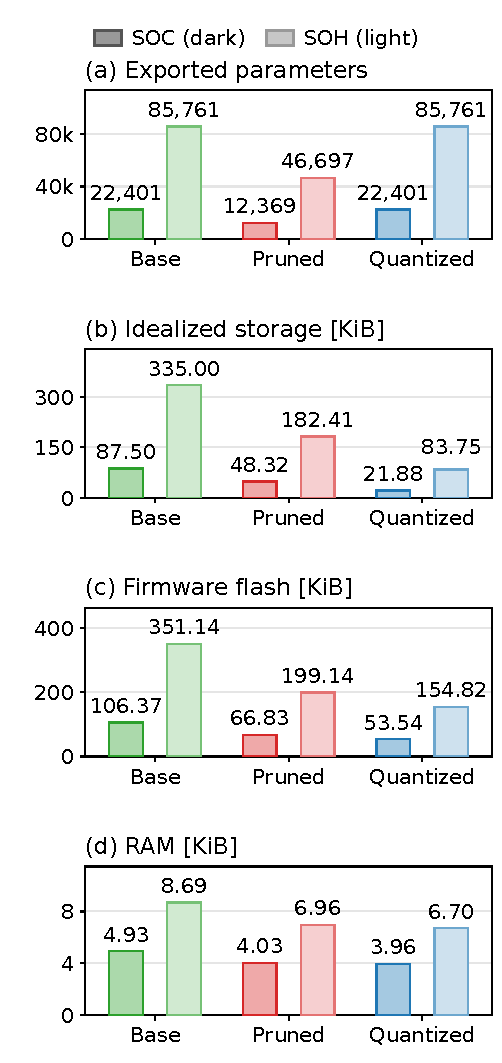
\includegraphics[width=\columnwidth]{gr14}
\end{figure}

\begin{figure}[,abovefloat=15pt,belowfloat=15pt]
\caption{\xlabel{fig:resources_latency}Latency distributions for SOC and SOH models on the STM32H7. Histograms are computed from repeated on-device measurements.}
\includegraphics[width=\columnwidth]{gr15}
\end{figure}

\subsection{Resource Efficiency and Latency}

\xref{fig:resources_sizes,fig:resources_latency} summarize the flash memory, RAM usage, parameter counts, and latency distributions for the SOC and SOH deployments on the STM32H7 microcontroller.
For all deployments the model complexity is first characterized by counting weights and biases in the exported C arrays. The two PyTorch LSTM bias vectors are merged during export, so each gate bias is counted once. Row scales added by quantization are storage metadata rather than learned parameters. Four bytes per parameter for Base and Pruned and one byte per parameter for Quantized define idealized storage estimates. Actual firmware flash is evaluated from the flash-backed loadable segments of the available STM32 executables, following the accounting described in \xref{sec:kpis}. Besides model constants, this footprint contains executable code, runtime support, and RAM initialization data. For Quantized, the difference from the all-INT8 estimate also reflects the retained FP32 biases, row scales, and MLP parameters. These distinct contributions explain why parameter storage and complete firmware occupancy should not be treated as interchangeable quantities.
The RAM values in panel (d) of \xref{fig:resources_sizes} use the same archived on-device records as \tabref{tab:kpi,tab:kpi_soh}. Initialized and zero-initialized static storage is added to the maximum stack usage recorded during streaming. For SOC, the resulting totals are 5048, 4124, and 4060 bytes for Base, Pruned, and Quantized, respectively. The corresponding SOH totals are 8896, 7128, and 6864 bytes. They describe the observed memory requirement of the evaluated replay. Pruning reduces the recurrent-state dimension, whereas weight-only quantization primarily reduces persistent matrix storage. Activations, hidden and cell states, biases, and the MLP remain FP32.
\xref{fig:resources_sizes} shows that Quantized produces the smallest flash footprint, while Pruned reduces both the parameter count and recurrent-state dimension. The measured RAM and execution-time results must nevertheless be considered separately because retaining FP32 activations and changing the kernel arithmetic prevents storage reduction from translating automatically into lower latency. \xref{fig:resources_latency} reports the corresponding host-side latency distributions.
The latency distributions in  \xref{fig:resources_latency} reveal a distinct hierarchy. SOC inference requires approximately \SIrange{0.8}{7}{\milli\second}, whereas the SOH variants require \SIrange{12}{30}{\milli\second} per update. The weight-quantized SOC deployment is slowest because the hand-written mixed-precision kernel applies FP32 row scales during the recurrent matrix products. When UART framing and host processing are included, end-to-end latencies remain below roughly \SI{20}{\milli\second} for SOC and \SI{50}{\milli\second} for SOH.



\subsection{Composite trade-off summary}

To make the multi-objective trade-offs easier to interpret at a glance, we report a composite utility score $U$ that aggregates accuracy and embedded resource indicators into a single, dimensionless index. For task-specific non-negative weights $\mathbf{w}=(w_A,w_F,w_R,w_E)$ with $\sum_j w_j=1$, model variant $v$ is scored as
\begin{equation}
\xlabel{eq:utility_u}
U_v(\mathbf{w}) =
w_A\frac{\mathrm{MAE}_v}{\mathrm{MAE}_{\mathrm{Base}}} +
w_F\frac{F_v}{F_{\mathrm{Base}}} +
w_R\frac{R_v}{R_{\mathrm{Base}}} +
w_E\frac{E_{\mathrm{est},v}}{E_{\mathrm{est,Base}}},
\end{equation}
where $\mathrm{MAE}$ is the streaming mean absolute error, $F$ is firmware flash from the executable audit, $R$ is recorded total RAM (static plus peak stack), and $E_{\mathrm{est}}$ is the timing-derived energy proxy. The main comparison uses equal weights, $w_A=w_F=w_R=w_E=0.25$. In this case, $U$ is the arithmetic mean of the four normalized objectives. Ratios, relative changes, and rankings are calculated before rounding the displayed memory and timing values. By construction $U_{\mathrm{Base}}=1$ for every valid weight vector. Lower values are preferred. Because $E_{\mathrm{est}}$ is proportional to inference time under the fixed-power assumption, the energy term represents timing priority rather than an independent power measurement.

Sensitivity is evaluated over all 1771 non-negative combinations on a 0.05 grid that sum to one. \xref{app:utility_sensitivity} also varies one highlighted objective from 25 to 85\%, sharing the remaining weight equally among the other three. Pruned is top-ranked for 93.85\% of SOC combinations and 53.36\% of SOH combinations. Quantized wins 6.15\% and 17.11\%, respectively, while Base wins 0\% for SOC and 29.53\% for SOH. The ranking is therefore robust for SOC Pruned but application-dependent for SOH: Base becomes preferable when accuracy dominates, whereas Quantized becomes preferable when flash receives high weight.
\tabref{tab:tradeoff_summary} summarizes the resulting changes for pruning and quantization. Values are reported as SOC/SOH.

\begin{table}[,abovefloat=15pt,belowfloat=15pt]%[width=0.8\textwidth]
\caption{\xlabel{tab:tradeoff_summary}At-a-glance effect of pruning and quantization relative to the corresponding Base model. Values are reported as SOC/SOH. $\Delta$MAE is reported in percentage points (pp) of full scale, where a negative value indicates improved accuracy. Flash, RAM, and estimated-energy changes are relative deltas versus Base. The composite score $U$ uses equal weights in~\neqref{eq:utility_u} (lower is better).}

\bstmfloatsrc
\begin{fsrc}
\tabcolsep=5.4pt
%\def\tblfont{\fontsize{6.5pt}{7.5pt}\selectfont}   %% re-define \tblfont if needed as per the layout
\tblfont
\begin{tabular*}{250pt}{lccccc}
        \toprule
        Variant & $\Delta$MAE [pp] & $\Delta$Flash [\%] & $\Delta$RAM [\%] & $\Delta E_{\mathrm{est}}$ [\%] & $U$ \\
        \midrule
        Pruned & \textcolor{mgGreen}{\tmin0.35}/\textcolor{mgRed}{+0.60} & \textcolor{mgGreen}{\tmin37}/\textcolor{mgGreen}{\tmin43} & \textcolor{mgGreen}{\tmin18}/\textcolor{mgGreen}{\tmin20} & \textcolor{mgGreen}{\tmin43}/\textcolor{mgGreen}{\tmin44} & 0.72/0.91 \\
        Quantized & \textcolor{mgRed}{+0.11}/\textcolor{mgRed}{+0.56} & \textcolor{mgGreen}{\tmin50}/\textcolor{mgGreen}{\tmin56} & \textcolor{mgGreen}{\tmin20}/\textcolor{mgGreen}{\tmin23} & \textcolor{mgRed}{+399}/\textcolor{mgRed}{+29} & 1.83/1.04 \\
        \bottomrule
    \end{tabular*}
\end{fsrc}
\estmfloatsrc

\end{table}

\subsection{Limited software fault sensitivity}

In the missing-output-report analysis, holding the preceding output for up to 10\% randomly unavailable reports changes aggregate MAE by less than 0.001 percentage points. Ten reporting gaps lasting 3600~s each increase SOC MAE by approximately 0.05 percentage points and have negligible influence on the slowly varying SOH output.

\xref{fig:app_fault_sensitivity} shows the recurrent response to the one-sample input-buffer faults. Across the SOC variants, median peak deviation ranges from 3.29 to 3.82 percentage points and P95 ranges from 16.18 to 23.81 percentage points. All 30 events per SOC model meet the recovery criterion within 60~s, with median recovery times of 10.0--12.5~s. Quantized follows Base closely, whereas Pruned has a lower median peak but the largest P95 peak. For SOH, median peak deviation ranges from 0.83 to 1.59 percentage points and P95 from 3.37 to 5.85 percentage points. The share recovered within 60~s is 93.3\% for Base, 90.0\% for Pruned, and 86.7\% for Quantized. Among the recovered SOH events, median recovery is 9, 7, and 5~s, respectively.

The target-based measure in Eq.~\neqref{eq:fault_mae_change} complements these disturbed-clean deviations. For SOC, median $\Delta\mathrm{MAE}_{61}$ ranges from 0.046 to 0.079 percentage points and P95 from 1.42 to 1.59 percentage points. For SOH, median changes lie between \tmin0.0009 and 0.0012 percentage points and P95 between 0.053 and 0.122 percentage points. The small negative SOH values occur when a disturbance moves an already imperfect prediction closer to the target and are not evidence of improved fault robustness. \tabref{tab:app_fault_mae} gives the model-specific values. The test therefore identifies different transient response tails across the compressed variants without indicating persistent SOC divergence or non-finite outputs. Its restricted fault location and event count do not support a hardware-safety claim.

\section{Discussion}

The experiments show that pruning and quantization affect the SOC and SOH estimators differently. For SOC, the evaluated Pruned model obtains a 0.35-percentage-point lower MAE than Base, while Quantized remains 0.11 percentage points above Base. Together with the L2 saliency and weight-distribution diagnostics, this identifies structured pruning as the more balanced transformation for the evaluated model and split. The experimental design uses one training run and a predefined test split for each task because the focus is the embedded comparison of compression routes. Repeated-seed validation, cross-validation, and matched unpruned fine-tuning can extend the statistical assessment of the observed advantage. The result is therefore reported without assigning it to a specific regularization mechanism.

For SOH the picture is more nuanced. Targets evolve slowly and are anchored by periodic capacity check-ups, while the displayed online estimates undergo two strong filtering stages. The filter-stage comparison shows that post-processing can alter not only absolute MAE but also the ranking between Base, Pruned, and Quantized. Compression quality should therefore be assessed on both raw and filtered outputs, and filter selection should consider response delay rather than MAE alone.

From an engineering perspective the three deployment variants represent distinct operating points. Base FP32 offers the simplest tool flow but requires the largest flash footprint. Pruning reduces the recurrent state dimension and the corresponding MLP input width, shrinking SOC flash from 106.37 to 66.83~KiB in the available builds. Recorded inference time decreases from 1.40 to 0.80~ms. For SOH the corresponding changes are 351.14 to 199.14~KiB and 22.73 to 12.72~ms. Within this unchanged FP32 kernel family, static MAC ratios and measured time ratios agree closely. SOC Pruned retains 54.9\% of Base MACs and 57.2\% of its time, while SOH retains 54.3\% and 56.0\%, respectively.

Weight-only quantization gives the smallest flash footprints,  \ubrk  53.54~KiB for SOC and 154.82~KiB for SOH, but changes the operation types without providing a fully integer execution path. Base and Quantized retain the same 22,080 SOC and 85,120 SOH model MACs. In the current C expressions, each recurrent INT8 weight is cast to FP32 and multiplied by its row scale inside the innermost accumulation, adding 17,920 source-level FP32 scale multiplications for SOC and 68,608 for SOH. Treating one MAC and one additional multiplication as one operation each gives a static Quantized/Base ratio of approximately 1.81 for both tasks, whereas the measured time ratios are 4.99 for SOC and 1.29 for SOH.

The discrepancy is expected because the count omits conversion, indexing, loop, load/store, nonlinear-function, and cache/Flash effects and because the \code{-O0} kernel uses no optimized integer dot-product path. For the larger SOH model, reduced recurrent-weight traffic may offset more of this arithmetic overhead than for SOC. Memory bandwidth was not measured, so this remains an implementation-based interpretation rather than a causal attribution. \xref{app:quant_runtime} places the static counts beside the measured DWT times.

The present kernel prioritizes a transparent implementation of the mixed-precision path. Potential improvements include accumulating each row before applying its shared scale, fusing scale and bias work, using DSP-optimized or integer dot-product kernels, and quantizing activations and recurrent states to enable a complete integer path. Operation-level cycle attribution and memory-bandwidth profiling are reserved for future implementation studies. The present results therefore establish total kernel timing for the tested firmware but not the fraction caused by conversion, arithmetic, or memory access.

The distinction between system latency, inference time, and estimated energy is particularly relevant for resource-constrained BMS. The UART-driven tests report end-to-end latency, while on-device inference spans 0.80--6.99~ms for SOC and 12.72--29.21~ms for SOH. The reported $E_{\mathrm{est}}$ values are obtained by multiplying these times by an assumed constant \SI{0.5}{\watt}. They do not isolate CPU, flash, SRAM, UART, or regulator contributions. Consequently, the results establish timing and memory trade-offs on the STM32H753ZI, but not a component-level energy budget or a conclusion that flash access dominates consumption.

The utility score makes the competing effects of compression directly comparable by expressing accuracy, flash, RAM, and the timing-derived energy proxy relative to the same Base model. A value below one indicates that the combined advantages outweigh the disadvantages for the selected priorities, while a value above one indicates an overall deterioration. With equal weights, $U=0.72$ identifies SOC Pruned as a balanced improvement, whereas $U=1.83$ shows that the flash reduction of SOC Quantized does not compensate for its timing overhead. The SOH scores of 0.91 for Pruned and 1.04 for Quantized remain close to one, indicating a genuine trade-off without one consistently dominant variant. The weight-grid analysis adds the important information of how stable these conclusions are when application priorities change. SOC Pruned remains preferred across most weight combinations, while the preferred SOH model depends more strongly on whether accuracy or flash receives greater emphasis. The utility analysis therefore supports a transparent selection of the model variant and distinguishes robust recommendations from priority-dependent decisions.

The implementation-level storage reduction follows directly from the architecture. Removing the same number of hidden channels or storing the same recurrent matrices as INT8 therefore produces predictable parameter-count changes for a fixed model topology. The preservation of estimation accuracy depends more strongly on the cell chemistry, operating conditions, reference construction, and training data. This study quantifies the trade-off for JGC LFP cells at \SI{25}{\degreeCelsius}. Existing embedded studies across different cell chemistries demonstrate that compact data-driven estimators are broadly feasible~\citep{giazitzisCaseStudyTiny2024,liOnlineCapacityEstimation2021,rzepkaNeuralNetworkArchitecture2023a}. Validation with additional cell chemistries is needed to determine how closely their attainable MAE and preferred compression level follow the trends observed here.

The present study examines two post-training compression routes. The first is one-shot structured pruning with short fine-tuning, and the second is recurrent-weight quantization of the original FP32 model. Quantization-aware training and pruning-aware or iterative training can in principle recover accuracy by adapting parameters to the imposed representation~\citep{krishnamoorthiQuantizingDeepConvolutional2018,wenLearningIntrinsicSparse2017}. Evaluating these strategies requires a separate training study and is reserved for future work. The current comparison therefore addresses deployable post-training transformations, not the best achievable result of jointly trained compression.

The analytical MAC relation provides a platform-independent estimate of how structured pruning changes model complexity. The measured flash and timing ratios complement this estimate for the evaluated STM32 implementation and build configuration. Their transfer to other embedded platforms depends on clock rate, floating-point and signal-processing support, compiler optimization, cache, and memory organization. Benchmarks on additional controller architectures can therefore quantify how these implementation characteristics translate the same model reduction into practical resource savings.

Preparing the derivative features on the host separates feature construction from neural-network inference and allows the measured timing differences to be attributed directly to pruning and quantization. The long-horizon analysis evaluates continuous inference trajectories, while the transient input-buffer analysis perturbs a measurement before inference and follows its effect through the recurrent state. The latter distinguishes immediate peak deviation, recovery, and target-MAE change. It indicates similar SOC behaviour for Base and Quantized, a larger upper-tail SOC response for Pruned, and a larger share of SOH events without confirmed 60-s recovery for Quantized. A complete embedded front-end and safety assessment can build on these results by additionally covering variable sampling, derivative filtering, recurrent-state and weight memory, activations, communication, and MCU memory.

\section{Conclusion and Outlook}

This study set out to quantify how two transparent compression routes change the accuracy and embedded cost of stateful SOC and SOH estimators under a common STM32 benchmark. Its contribution is an auditable comparison from trained LSTM\,+\,MLP models to continuous C inference with consistent accuracy, memory, and timing indicators. Estimated energy per inference remains a constant-power timing proxy and is not an independent power measurement.

For SOC, Pruned reduces flash by 37.2\%, RAM by approximately 18\%, and inference time by 42.9\%, while its MAE is 0.35 percentage points lower than Base for the evaluated model and split. Quantized reduces flash by 49.7\% and RAM by approximately 20\%, but increases inference time by 399\% and MAE by 0.11 percentage points in the mixed-precision software kernel. For SOH, Pruned reduces flash by 43.3\%, RAM by approximately 20\%, and inference time by 44.0\%, with a 0.60-percentage-point MAE increase. Quantized reduces flash by 55.9\% and RAM by approximately 23\%, while increasing inference time by 28.5\% and MAE by 0.56 percentage points. Under the fixed-power assumption, the energy proxy changes by the same percentages as inference time.

These results identify structured pruning as the more balanced operating point for the tested firmware, whereas recurrent-weight quantization is attractive primarily when flash capacity dominates and its dequantization overhead is acceptable. Ten consecutive replay segments show no quantization-specific monotonic deviation from Base. After transient input-buffer bit flips, every SOC variant recovers in all 30 events within 60~s, while 6.7--13.3\% of the SOH events do not meet the defined recovery criterion within this horizon. The SOH filter analysis further shows that compression must be assessed together with post-processing delay. The evaluated LFP trajectories, model configurations, STM32H753ZI implementation, and compiler settings establish the trade-off under one complete deployment scenario. Validation across additional cell chemistries, embedded platforms, model initializations, and internal fault classes can determine how broadly the observed trends transfer.

The first priority for future work is to optimize and profile the mixed-precision kernel through row-scale hoisting, operator fusion, DSP-oriented dot products, and activation/state quantization, while measuring per-model board power with external instrumentation. A second priority is external validation across random seeds, temperatures, cell chemistries, and embedded platforms, including direct comparison with quantization-aware and pruning-aware training. Finally, internal weight, activation, recurrent-state, sensor, communication, and MCU fault injection is required before safety-related claims can be made. Joint pruning and quantization remains a promising route for combining a reduced state dimension with compact recurrent storage.

\printauthorcredits

\beginAIdeclaration[Declaration of generative AI and  AI-assisted technologies in the manuscript preparation process]
During the preparation of this work the author(s) used ChatGPT, DeepL, and Grammarly in order to improve the linguistic quality and style of the manuscript. After using these tools, the author(s) reviewed and edited the content as needed and take(s) full responsibility for the content of the published article.
\endAIdeclaration
\printAIsection

\conflictofinterest

\DoCIyes{Julia Kowal reports financial support was provided by German Federal Ministry for Education and Research (BMBF). Julia Kowal reports financial support was provided by German Research Foundation. Julia Kowal reports financial support was provided by Open Access Publication Fund of the Technical University of Berlin. If there are other authors, they declare that they have no known competing financial interests or personal relationships that could have appeared to influence the work reported in this paper.}

\ukackheads

This research was funded by the \grantsponsor{German Federal Ministry for Education
and Research (BMBF)}[http://dx.doi.org/10.13039/501100002347], grant number \grantnumber{1}{03SF0684A} (MG FARM). The authors
are responsible for the content. The work was further supported by the \grantsponsor{German
Research Foundation and the Open Access Publication Fund of the Technical
University of Berlin}. We acknowledge the High Performance Computing Service of the Technical University of Berlin for providing the computational resources used in the pruning and quantization experiments. The authors thank Nils Strassenburg (Hasso-Plattner-Institut, Potsdam) for helpful discussions on pruning and quantization, Mano Schmitz for the collaboration on the dataset creation, and Max M{\"o}nikes and Pavel Aleinikau (Technical University of Berlin) for their collaboration on the BMS hardware. 
%\QUERY[4]
%\QUERY[5]
\appendix{}
\section[pfx={Appendix},nonum]{Supplementary compression and robustness analyses}\xlabel{app:supplementary}

This appendix presents supporting analyses of pruning structure, temporal stability, filter interaction, utility sensitivity, transient input faults, model-complexity scaling, mixed precision, and kernel operation counts.

\subsection{Structured-pruning diagnostics}\xlabel{app:pruning_diagnostics}

See \xref{TeXFolio:figA.16}.

\begin{figure*}[,abovefloat=165pt,belowfloat=155pt]
\caption{\xlabel{fig:app_pruning_diagnostics}Diagnostics for the one-shot SOC pruning operation. (a) L2 saliency from Eq.~\neqref{eq:pruning_saliency}, sorted in ascending order. The 19 lowest-ranked units are removed and 45 units are retained. (b) Density of the central recurrent-weight range for the Base and Pruned models. The analysis confirms application of the specified ranking criterion and makes the resulting weight selection transparent. Repeated training runs can extend this structural evidence towards a statistical assessment of the observed MAE difference.}
\includegraphics{gr16}
\end{figure*}

\subsection{Long-horizon temporal stability}\xlabel{app:long_horizon}

See \xref{TeXFolio:figA.17}.

\begin{figure*}[,abovefloat=15pt]
\caption{\xlabel{fig:app_long_horizon}Temporal error and model-to-Base deviation over ten consecutive, equal-count segments of the full-stream replay. Recurrent states are not reset at segment boundaries. Panels (a) and (c) show target MAE for SOC and SOH. Panels (b) and (d) show the mean absolute deviation of Pruned and Quantized from Base. The absence of monotonic late-sequence divergence demonstrates stable relative behaviour across the complete evaluated replay. Further sequences can extend the tested operating horizon.}
\includegraphics{gr17}
\end{figure*}

\subsection{{\?{SOH}} filtering and compression interaction}\xlabel{app:soh_filter}

See \xref{TeXFolio:figA.18}.

\begin{figure*}[,abovefloat=11pt]
\caption{\xlabel{fig:app_soh_filter}Comparison of SOH compression and filtering for the Base, Pruned, and Quantized C models on a common input sequence. (a) Outputs after first-point alignment but before temporal filtering. (b) Stage~1 with $\alpha_1=0.02$ and the symmetric limiter. (c) Final sequential output after applying stage~2 with $\alpha_2=10^{-6}$ and the downward limiter to stage~1. (d) MAE after each processing stage. At \SI{1}{\hertz}, the EMA-only 90\% response times are approximately \SI{114}{\second} and 26.65~days, respectively. The nonlinear limiters have no single cutoff frequency. All three variants use the same input and processing order to isolate the interaction between compression and filtering.}
\includegraphics[scale=0.9]{gr18}
\end{figure*}

\subsection{Utility-weight sensitivity}\xlabel{app:utility_sensitivity}

See \xref{TeXFolio:figA.19}.

\begin{figure*}
\caption{\xlabel{fig:app_utility_sensitivity}Sensitivity of the utility ranking to application priorities. Panels (a) and (b) vary the highlighted objective from 25 to 85\% and divide the remaining weight equally among the other three objectives. Each square identifies the lowest-utility model. At 25\%, all four objectives have equal weight. Panel (c) gives the winning share across all 1771 non-negative 0.05-spaced weight combinations that sum to one. The energy objective uses the timing-derived $E_{\mathrm{est}}$ proxy and is therefore not an independent power measurement.}
\includegraphics[width=\textwidth]{gr19}
\end{figure*}

\subsection{Transient input-buffer fault sensitivity}\xlabel{app:fault_sensitivity}

See \xref{TeXFolio:figA.20}.

\begin{figure*}
\caption{\xlabel{fig:app_fault_sensitivity}Stateful response to transient software input-buffer corruption. Thirty independent events per task and model flip bit~22, the highest-order FP32 fraction bit, in voltage, current, or temperature for one 1-Hz sample, with ten events per input signal. The clean and disturbed branches start from the same recurrent state and then receive the same 60 unmodified follow-up inputs, corresponding to 60~s, without a state reset. (a) and (b) show the absolute disturbed-clean deviation for one representative voltage event. (c) summarizes the median peak and P95 peak across all 30 events. (d) gives the fraction that meets the sustained recovery criterion within 60~s. The figure characterizes propagation through the recurrent state, while \tabref{tab:app_fault_mae} reports the corresponding change in target MAE.}
\includegraphics{gr20}
\end{figure*}

See \tabref{TeXFolio:tabA.4}.

\def\thetable{A.\arabic{table}}
\begin{table}[,abovefloat=15pt,belowfloat=15pt]%[width=0.8\textwidth]
\caption{\xlabel{tab:app_fault_mae}Change in target MAE over the window comprising one corrupted sample and 60 clean follow-up samples. Values are percentage points and summarize 30 independent input-bitflip events per task and model. The change is defined by Eq.~\neqref{eq:fault_mae_change}. Negative values indicate that the disturbed output happens to lie closer to the target in part of the window.}


\begin{tabular}{LLRL}
\beginthead
Task & Model & \multicolumn{1}{L}{Median $\Delta\mathrm{MAE}_{61}$ [pp]} & P95 $\Delta\mathrm{MAE}_{61}$ [pp] \\
\endthead\rowhead 
SOC & Base      & 0.0740  & 1.4235 \\
SOC & Pruned    & 0.0464  & 1.5867 \\
SOC & Quantized & 0.0785  & 1.4314 \\
SOH & Base      & \tmin0.0009 & 0.1224 \\
SOH & Pruned    & \tmin0.00004 & 0.0533 \\
SOH & Quantized & 0.0012  & 0.1055 
\botline
\end{tabular}
\end{table}

\subsection{Analytical model-complexity scaling}\xlabel{app:model_complexity}

See \xref{TeXFolio:figA.21}.

\begin{figure*}[,abovefloat=75pt,belowfloat=55pt]
\caption{\xlabel{fig:app_model_complexity}Architecture-level operation scaling from Eq.~\neqref{eq:model_macs}. (a) Analytical MACs per streaming inference over LSTM hidden size, with markers for the implemented SOC and SOH Base and Pruned dimensions. (b) Finite-model reduction for the evaluated pruning fraction $p=0.30$, including the implemented SOC and SOH points and the 51\% large-$H$ limit. (c) General relation between the hidden-unit pruning fraction and the asymptotic reduction $2p-p^2$. The highlighted 30\% operating point has a theoretical limit of 51\%, while the corresponding limits for 10, 20, 40, and 50\% pruning are 19, 36, 64, and 75\%. Linear input and MLP terms together with the fixed output term keep finite models below the respective limit.}
\includegraphics{gr21}
\end{figure*}

\subsection{Scope of the \?{L2} pruning criterion}\xlabel{app:pruning_criterion_scope}

See \xref{TeXFolio:figA.22}.

\begin{figure*}[,abovefloat=55pt]
\caption{\xlabel{fig:app_pruning_criterion_scope}Scope of the structured pruning criterion. (a) Normalized L2 saliency ranks for the SOC and SOH Base hidden units. The lowest 30\% define the task-specific removal sets. (b) The implemented path aggregates row-wise L2 norms across all four gates and removes complete recurrent units together with associated recurrent columns and MLP inputs. The comparison makes the reproducibility and dense-kernel benefit of the L2 criterion explicit and provides a reference for future comparisons with gradient- and activation-based rankings.}
\includegraphics{gr22}
\end{figure*}

\subsection{Verified mixed-precision boundary}\xlabel{app:mixed_precision}

See \xref{TeXFolio:figA.23}.

\begin{figure*}[,abovefloat=55pt]
\caption{\xlabel{fig:app_mixed_precision}Verified precision path and raw model-constant composition. (a) Only recurrent input-to-hidden and hidden-to-hidden matrices are stored as INT8. Per-row scales, biases, gate activations, hidden/cell states, the MLP, and the estimator output remain FP32. (b,c) Analytical model constants for SOC and SOH Base and Quantized variants. The comparison shows how concentrating quantization on the dominant recurrent matrices reduces persistent model storage and where activation and state quantization could provide additional runtime savings.}
\includegraphics{gr23}
\end{figure*}

\subsection{Static quantized-runtime accounting}\xlabel{app:quant_runtime}

See \xref{TeXFolio:figA.24}.

\begin{figure*}
\caption{\xlabel{fig:app_quant_runtime}Static source-level operation accounting beside measured STM32H753ZI kernel time. Panels (a,c) show model MACs and the additional FP32 row-scale multiplications implied by the current per-weight C expressions. Panels (b,d) show DWT measurements averaged over 10,000 streaming inferences. Their comparison reveals where analytical operation counts explain the timing trend and where conversion, indexing, loop, load/store, nonlinear-function, compiler, and memory-system effects create additional optimization opportunities.}
\includegraphics{gr24}
\end{figure*}

\text{}

\back{}

\bibliographystyle{stm-xml-sort-names-fnm-abre-v1}

\nocite{*}

\bibliography{\jobname.bib}


\begin{bibwrite}{\jobname.bib}

@preamble{"\tfbibfldoff[issn,isbn]"}

@article{yaoSmarterBatteryManagement2025a,

SerialNo={1},
author={Yao, Jiaqi and Kowal, Julia},
year={2025},
title={Towards a Smarter Battery Management System: \?{A} Critical Review on
Deep Learning-Based State of Charge Estimation of Lithium-Ion Batteries},
journal={Energy AI},
volume={21},
artnum={100585},
doi={10.1016/j.egyai.2025.100585},
issn={26665468},
xdateaccessed={2025-12-04},
}
%\QUERY[6]
@article{a.m.s.m.h.s.attanayakaEstimationStateCharge2019,
SerialNo={2},

author={{A. M. S. M. H. S. Attanayaka}, {} and {J. P. Karunadasa}, {} and {K. T. M. U.
Hemapala}, {} and {Department of Electrical Engineering, University of Moratuwa,
Moratuwa, Sri Lanka}, {}},
year={2019},
title={Estimation of State of Charge for Lithium-Ion Batteries - {{A
Review}}},
journal={AIMS Energy},
volume={7},
number={2},
pages={186--210},
doi={10.3934/energy.2019.2.186},
issn={2333-8334},
xdateaccessed={2025-12-02},
}

@article{berecibarCriticalReviewState2016,
SerialNo={3},
author={Berecibar, M. and Gandiaga, I. and Villarreal, I. and Omar, N. and Van
Mierlo, J. and Van Den Bossche, P.},
year={2016},
title={Critical Review of State of Health Estimation Methods of {{Li-ion}}
Batteries for Real Applications},
journal={{\rvtissnRenewable} {\rvtissnSustain} Energy {\rvtissnReview}},
volume={56},
pages={572--587},
doi={10.1016/j.rser.2015.11.042},
issn={13640321},
xdateaccessed={2025-12-02},
}

@article{shrivastavaReviewTechnologicalAdvancement2023,
SerialNo={4},
author={Shrivastava, Prashant and Naidu, P. Amritansh and Sharma, Sakshi and
Panigrahi, Bijaya Ketan and Garg, Akhil},
year={2023},
title={Review on Technological Advancement of Lithium-Ion Battery States
Estimation Methods for Electric Vehicle Applications},
journal={{\rvtissnJournal} Energy Storage},
volume={64},
artnum={107159},
doi={10.1016/j.est.2023.107159},
issn={2352152X},
xdateaccessed={2025-01-14},
keywords={ML besser als andere},
}

@article{guoSystematicReviewElectrochemical2024,
SerialNo={5},
author={Guo, Feng and Couto, Luis D. and Mulder, Grietus and Trad, Khiem and
Hu, Guangdi and Capron, Odile and Haghverdi, Keivan},
year={2024},
title={A Systematic Review of Electrochemical Model-Based Lithium-Ion Battery
State Estimation in Battery Management Systems},
journal={{\rvtissnJournal} Energy Storage},
volume={101},
artnum={113850},
doi={10.1016/j.est.2024.113850},
issn={2352152X},
xdateaccessed={2025-01-14},
keywords={Ubersicht SOC und SOH Bestimmung},
}
%\QUERY[7]
@others{leap-reMGFARMSmart,
SerialNo={6},
author={{LEAP-RE}, {}},
year={0000},
commn={(0000), {{\?{MG} \?{FARM} Smart}} Stand-Alone Micro-Grids as a Solution for Agriculture   Farms Electrification,  \myehost{https://www.leap-re.eu/mg-farm/}},
}

@others{microenergyMGFARMPoweringSustainable,
SerialNo={7},
author={Microenergy, {}},
year={0000},
commn={{{\?{MG}-\?{FARM} Powering Sustainable Agriculture}} with {{Smart   Micro-Grids}}, \myehost{https://mg-farm.microenergy-consulting.com/}},
}

@inbook{aqachtoulMGFARMIoTEdgeDriven2026,
SerialNo={8},
author={Aqachtoul, A. and Karam, K. and Elamrani, A. and Alidrissi, Y. and
Najib, M. and Rochd, A. and Bakhouya, M.},
year={2026},
title={{{\?{MGFARM}}}: {{An \?{IoT}}} and {{Edge-Driven Framework}} for {{Smart}} and
{{Sustainable Agricultural Practices}}},
booktitle={Connected {{Objects}}, {{Artificial Intelligence}},
{{Telecommunications}} and {{Electronics Engineering}}},
volume={vol. 1584},
pages={419--425},
orgname={Springer Nature Switzerland},
city = {Cham},
editor={Mejdoub, Youssef and Elamri, Abdelkebir and Kardouchi, Mustapha},
doi={10.1007/978-3-032-01536-5\_64},
isbn={978-3-032-01535-8 978-3-032-01536-5},
xdateaccessed={2025-12-03},
}

@others{technischeuniversitatberlinMGFarmSmart,
SerialNo={9},
author={{Technische Universit{\"a}t Berlin}, {}},
year={0000},
commn={{{\?{MG} Farm Smart}} Microgrids as a Solution for Agriculture Farms   Electrification,  \myehost{https://www.tu.berlin/eet/forschung/projekte/mg-farm}},
}

@article{crocioniLiIonBatteriesParameter2020,
SerialNo={10},
author={Crocioni, Giulia and Pau, Danilo and Delorme, Jean-Michel and Gruosso,
Giambattista},
year={2020},
title={Li-{{Ion Batteries Parameter Estimation With Tiny Neural Networks
Embedded}} on {{Intelligent {\?{IoT}} Microcontrollers}}},
journal={IEEE Access},
volume={8},
pages={122135--122146},
doi={10.1109/ACCESS.2020.3007046},
issn={2169-3536},
xdateaccessed={2025-05-19},
}

@article{giazitzisCaseStudyTiny2024,
SerialNo={11},
author={Giazitzis, Spyridon and Sakwa, Maciej and Leva, Sonia and Ogliari,
Emanuele and Badha, Susheel and Rosetti, Filippo},
year={2024},
title={A {{case study}} of a {{tiny machine learning application}} for
{{battery state-of-charge estimation}}},
journal={Electronics},
volume={13},
number={10},
pages={1964},
doi={10.3390/electronics13101964},
issn={2079-9292},
xdateaccessed={2025-05-19},
keywords={Embedded AI},
}

@article{Embedded_AI_only_SOC_mobile,
SerialNo={12},
author={Pau, Danilo Pietro and Aniballi, Alberto},
year={2024},
title={Tiny {{machine learning battery state-of-charge estimation hardware
accelerated}}},
journal={\rvtsclApplSci},
volume={14},
number={14},
pages={6240},
doi={10.3390/app14146240},
issn={2076-3417},
xdateaccessed={2025-05-19},
keywords={Embedded AI,Microcontroller,SOC},
}

@article{Embedded_AI_SOH_badData,
SerialNo={13},
author={Kamali, M. Adib and Caliwag, Angela C. and Lim, Wansu},
year={2021},
title={Novel {{\?{SOH} estimation}} of {{lithium-ion batteries}} for {{real-time
embedded applications}}},
journal={IEEE {\rvtissnEmbed} {\rvtissnSystem} {\rvtissnLetter}},
volume={13},
number={4},
pages={206--209},
doi={10.1109/LES.2021.3078443},
issn={1943-0663, 1943-0671},
xdateaccessed={2025-05-19},
keywords={Embedded AI,Microcontroller,SOH},
}

@inbook{naguibMicroprocessorExecutionTime2022,
SerialNo={14},
author={Naguib, Mina and Kollmeyer, Phillip and Vidal, Carlos and Duque,
Josimar and Gross, Oliver and Emadi, Ali},
year={2022},
title={Microprocessor {{execution time}} and {{memory use}} for {{battery
state}} of {{charge estimation algorithms}}},
booktitle={{{WCX SAE World Congress Experience}}},
pages={2022--01--0697},
city = {Detroit \& Online, Michigan, United States},
doi={10.4271/2022-01-0697},
xdateaccessed={2025-12-03},
}

@CUSTOMBIB{LFP_DoE_Cycle_Aging_Dataset,
mypattern={[authors,atitle,midc][booktag,bktitle,yr,endbooktag,bibpages,bibdoi][post,myehost]},
SerialNo={15},
author={Rzepka, Florian},
year={2025},
title={Design of {{experiments}} for {{cyclic aging}} of {{\?{LFP}}} 18650
{{Cells}}: {{Impact}} of {{Charge}}/\?{{{Discharge} \?{C}-Rates}}, {{Depth}} of
{{Discharge}}, and {{Temperature}} on {{Battery Degradation}}},
orgname={Technische Universit\"at Berlin},
doi={10.14279/DEPOSITONCE-24800},
xdateaccessed={2025-12-02},
keywords={18650,battery aging,cyclic aging,Design of Experiments (DoE),Lithium
Iron Phosphate (LFP)},
}

@article{wang_improved_2024,
SerialNo={16},
author={Wang, Shunli and Wang, Chao and Takyi-Aninakwa, Paul and Jin, Siyu and
Fernandez, Carlos and Huang, Qi},
year={2024},
title={An improved parameter identification and radial basis
correction-differential support vector machine strategies for state-of-charge
estimation of urban-transportation-electric-vehicle lithium-ion batteries},
journal={{\rvtissnJournal} Energy Storage},
volume={80},
artnum={110222},
doi={10.1016/j.est.2023.110222},
issn={2352152X},
xdateaccessed={2026-07-15},
post={\xURL \myehost{https://linkinghub.elsevier.com/retrieve/pii/S2352152X23036216}},
}

@article{wang_improved_2023,
SerialNo={17},
author={Wang, Shunli and Wu, Fan and Takyi-Aninakwa, Paul and Fernandez,
Carlos and Stroe, Daniel-Ioan and Huang, Qi},
year={2023},
title={Improved singular filtering-{\?{Gaussian}} process regression-long
short-term memory model for whole-life-cycle remaining capacity estimation of
lithium-ion batteries adaptive to fast aging and multi-current variations},
journal={Energy},
volume={284},
artnum={128677},
doi={10.1016/j.energy.2023.128677},
issn={03605442},
xdateaccessed={2026-07-15},
post={\xURL \myehost{https://linkinghub.elsevier.com/retrieve/pii/S0360544223020716}},
}

@article{gaoCoEstimationStateofChargeStateof2022,
SerialNo={18},
author={Gao, Yizhao and Liu, Kailong and Zhu, Chong and Zhang, Xi and Zhang,
Dong},
year={2022a},
title={Co-{{estimation}} of {{state-of-charge}} and {{state-of- health}} for
{{lithium-ion batteries using}} an {{enhanced electrochemical model}}},
journal={\rvtiopIEEETransIndElectron},
volume={69},
number={3},
pages={2684--2696},
doi={10.1109/TIE.2021.3066946},
issn={0278-0046, 1557-9948},
xdateaccessed={2025-01-14},
keywords={Combined SOC and SOH Estimation},
}

@article{gaoEnhancedStateofchargeEstimation2022,
SerialNo={19},
author={Gao, Yizhao and Plett, Gregory L. and Fan, Guodong and Zhang, Xi},
year={2022b},
title={Enhanced State-of-Charge Estimation of {{{\?{LiFePO4}}}} Batteries Using an
Augmented Physics-Based Model},
journal={\rvtiopJPowerSources},
volume={544},
artnum={231889},
doi={10.1016/j.jpowsour.2022.231889},
issn={03787753},
xdateaccessed={2025-01-14},
keywords={SOC Estimation},
}

@article{shenAlternativeCombinedCoestimation2022,
SerialNo={20},
author={Shen, Jiangwei and Ma, Wensai and Xiong, Jian and Shu, Xing and Zhang,
Yuanjian and Chen, Zheng and Liu, Yonggang},
year={2022},
title={Alternative Combined Co-Estimation of State of Charge and Capacity for
Lithium-Ion Batteries in Wide Temperature Scope},
journal={Energy},
volume={244},
artnum={123236},
doi={10.1016/j.energy.2022.123236},
issn={03605442},
xdateaccessed={2025-01-14},
keywords={Combined SOC and SOH Estimation},
}

@article{wangFusionEstimationLithiumion2022,
SerialNo={21},
author={Wang, Chunyu and Cui, Naxin and Cui, Zhongrui and Yuan, Haitao and
Zhang, Chenghui},
year={2022},
title={Fusion Estimation of Lithium-Ion Battery State of Charge and State of
Health Considering the Effect of Temperature},
journal={{\rvtissnJournal} Energy Storage},
volume={53},
artnum={105075},
doi={10.1016/j.est.2022.105075},
issn={2352152X},
xdateaccessed={2025-01-14},
keywords={Combined SOC and SOH Estimation},
}

@inbook{sunStateChargeEstimation2023,
SerialNo={22},
author={Sun, Wenjie and Zhou, Bangyu and Xu, Huan and Yao, Wenjiao and Guo,
Yuanjun and Yang, Zhile},
year={2023},
title={State of {{Charge Estimation}} of {{Sodium-Ion Batteries Based}} on
{{N-\?{BEATS} Neural Network}}},
booktitle={2023 7th {{Asian Conference}} on {{Artificial Intelligence
Technology}} ({{ACAIT}})},
pages={1395--1401},
orgname={IEEE},
city = {Jiaxing, China},
doi={10.1109/ACAIT60137.2023.10528411},
isbn={979-8-3503-5914-5},
xdateaccessed={2025-01-13},
keywords={nur SOC,Sodium},
}

@article{sunStateofchargeEstimationSodiumion2024,
SerialNo={23},
author={Sun, Wenjie and Xu, Huan and Zhou, Bangyu and Guo, Yuanjun and Tang,
Yongbing and Yao, Wenjiao and Yang, Zhile},
year={2024},
title={State-of-Charge Estimation of Sodium-Ion Batteries: \?{A} Fusion Deep
Learning Approach},
journal={{\rvtissnJournal} Energy Storage},
volume={91},
artnum={111527},
doi={10.1016/j.est.2024.111527},
issn={2352152X},
xdateaccessed={2025-01-13},
keywords={nur SOC},
}

@article{liOnlineCapacityEstimation2021,
SerialNo={24},
author={Li, Weihan and Sengupta, Neil and Dechent, Philipp and Howey, David
and Annaswamy, Anuradha and Sauer, Dirk Uwe},
year={2021},
title={Online Capacity Estimation of Lithium-Ion Batteries with Deep Long
Short-Term Memory Networks},
journal={\rvtiopJPowerSources},
volume={482},
artnum={228863},
doi={10.1016/j.jpowsour.2020.228863},
issn={03787753},
xdateaccessed={2025-01-14},
keywords={SOH Estimation},
}
%\QUERY[8]
@others{ONNXRuntimeHighperformance,
SerialNo={25},
author={{ONNX Runtime}, {}},
year={0000},
commn={{{\?{ONNX} Runtime}}: \?{H}igh-Performance Inference Engine, \myehost{https://onnxruntime.ai/}},
}

@others{NVIDIATensorRTHighPerformance,
SerialNo={26},
author={{NVIDIA TensorRT}, {}},
year={0000},
commn={{{\?{NVIDIA} TensorRT}}: {{High-Performance Deep Learning Inference}},  \myehost{https://developer.nvidia.com/tensorrt}},
}

@others{XCUBEAISTM32CubeExpansion,
SerialNo={27},
author={{X-CUBE-AI}, {}},
year={0000},
commn={(0000), X-{{\?{CUBE}-\?{AI}}}: {{\?{STM}32Cube Expansion Package}} for {{Artificial   Intelligence}}, \myehost{https://www.st.com/en/embedded-software/x-cube-ai.html}},
}

@inbook{schulzePQBenchBenchmarking2025,
SerialNo={28},
author={Schulze, Jonas and Strassenburg, Nils and Rabl, Tilmann},
year={2025},
title={{{\?{PQ} Bench}}: {{Benchmarking pruning}} and {{quantization
techniques}}},
booktitle={Proceedings of the {{Workshop}} on {{Data Management}} for
{{End-To-End Machine Learning}}},
pages={1--6},
orgname={ACM},
city = {Berlin Germany},
doi={10.1145/3735654.3735940},
isbn={979-8-4007-1924-0},
xdateaccessed={2025-12-05},
}

@others{jgneJGCFR186501800mAh32VProductSpecification,
SerialNo={29},
author={{JGNE}, {}},
year={0000},
commn={(0000), {{\?{JGCFR}18650-1800mAh-{\?{3}}}}.{{{\?{2V}} Product Specification}}},
orgname={JGNE},
}

@article{kucevicStandardBatteryEnergy2020a,
SerialNo={30},
author={Kucevic, Daniel and Tepe, Benedikt and Englberger, Stefan and
Parlikar, Anupam and M{\"u}hlbauer, Markus and Bohlen, Oliver and Jossen,
Andreas and Hesse, Holger},
year={2020},
title={Standard Battery Energy Storage System Profiles: {{Analysis}} of
Various Applications for Stationary Energy Storage Systems Using a Holistic
Simulation Framework},
journal={{\rvtissnJournal} Energy Storage},
volume={28},
artnum={101077},
doi={10.1016/j.est.2019.101077},
issn={2352152X},
xdateaccessed={2025-12-15},
}

@book{siebertzStatistischeVersuchsplanung2017,
SerialNo={31},
author={Siebertz, Karl and Van Bebber, David and Hochkirchen, Thomas},
year={2017},
booktitle={{Statistische Versuchsplanung}},
orgname={Springer Berlin Heidelberg},
city = {Berlin, Heidelberg},
doi={10.1007/978-3-662-55743-3},
isbn={978-3-662-55742-6 978-3-662-55743-3},
xdateaccessed={2025-12-03},
aetag={\xvfill\xeject},
}

@inbook{huberRobustStatistics2009,
SerialNo={32},
author={Huber, Peter J. and Ronchetti, Elvezio M.},
year={2009},
title={Robust {{Statistics}}},
series={Wiley {{Series}} in {{Probability}} and {{Statistics}}},
edition={first ed.},
orgname={Wiley},
doi={10.1002/9780470434697},
isbn={978-0-470-12990-6 978-0-470-43469-7},
xdateaccessed={2025-12-02},
}

@CUSTOMBIB{pedregosaScikitlearnMachineLearning2012,
mypattern={[authors,atitle,midc][booktag,bktitle,yr,endbooktag,bibpages,bibdoi][post,myehost]},
SerialNo={33},
author={Pedregosa, Fabian and Varoquaux, Ga{\"e}l and Gramfort, Alexandre and
Michel, Vincent and Thirion, Bertrand and Grisel, Olivier and Blondel,
Mathieu and M{\"u}ller, Andreas and Nothman, Joel and Louppe, Gilles and
Prettenhofer, Peter and Weiss, Ron and Dubourg, Vincent and Vanderplas, Jake
and Passos, Alexandre and Cournapeau, David and Brucher, Matthieu and Perrot,
Matthieu and Duchesnay, {\'E}douard},
year={2012},
title={Scikit-Learn: {{Machine Learning}} in {{Python}}},
orgname={arXiv},
doi={10.48550/ARXIV.1201.0490},
xdateaccessed={2025-12-02},
keywords={FOS: Computer and information sciences,Machine Learning
(cs.LG),Mathematical Software (cs.MS)},
}

@inbook{plettBatteryManagementSystems2015,
SerialNo={34},
author={Plett, Gregory L.},
year={2015},
title={Battery Management Systems: {{Volume}} {\?{1}}: \?{B}attery Modeling},
series={Artech {{House}} Power Engineering and Power Electronics},
orgname={Artech House},
city = {Boston London},
isbn={978-1-63081-024-5},
}

@CUSTOMBIB{liptonCriticalReviewRecurrent2015,
mypattern={[authors,atitle,midc][booktag,bktitle,yr,endbooktag,bibpages,bibdoi][post,myehost]},
SerialNo={35},
author={Lipton, Zachary C. and Berkowitz, John and Elkan, Charles},
year={2015},
title={A {{Critical Review}} of {{Recurrent Neural Networks}} for {{Sequence
Learning}}},
orgname={arXiv},
doi={10.48550/ARXIV.1506.00019},
xdateaccessed={2025-12-02},
keywords={FOS: Computer and information sciences,Machine Learning
(cs.LG),Neural and Evolutionary Computing (cs.NE)},
}

@CUSTOMBIB{paszkePyTorchImperativeStyle2019,
mypattern={[authors,atitle,midc][booktag,bktitle,yr,endbooktag,bibpages,bibdoi][post,myehost]},
SerialNo={36},
author={Paszke, Adam and Gross, Sam and Massa, Francisco and Lerer, Adam and
Bradbury, James and Chanan, Gregory and Killeen, Trevor and Lin, Zeming and
Gimelshein, Natalia and Antiga, Luca and Desmaison, Alban and K{\"o}pf,
Andreas and Yang, Edward and DeVito, Zach and Raison, Martin and Tejani,
Alykhan and Chilamkurthy, Sasank and Steiner, Benoit and Fang, Lu and Bai,
Junjie and Chintala, Soumith},
year={2019},
title={{{PyTorch}}: {{An imperative style}}, {{high-performance deep learning
library}}},
xnumber={arXiv:1912.01703},
xorgname={arXiv},
post={\myehost{http://arxiv.org/abs/1912.01703}[arXiv:1912.01703]},
primaryClass={cs},
doi={10.48550/arXiv.1912.01703},
xdateaccessed={2025-12-02},
keywords={Computer Science - Machine Learning,Computer Science - Mathematical
Software,Statistics - Machine Learning},
}

@CUSTOMBIB{loshchilovDecoupledWeightDecay2017,
mypattern={[authors,atitle,midc][booktag,bktitle,yr,endbooktag,bibpages,bibdoi][post,myehost]},
SerialNo={37},
author={Loshchilov, Ilya and Hutter, Frank},
year={2017},
title={Decoupled {{Weight Decay Regularization}}},
orgname={arXiv},
doi={10.48550/ARXIV.1711.05101},
xdateaccessed={2025-12-02},
keywords={FOS: Computer and information sciences,FOS: Mathematics,Machine
Learning (cs.LG),Neural and Evolutionary Computing (cs.NE),Optimization and
Control (math.OC)},
}

@CUSTOMBIB{loshchilovSGDRStochasticGradient2016,
mypattern={[authors,atitle,midc][booktag,bktitle,yr,endbooktag,bibpages,bibdoi][post,myehost]},
SerialNo={38},
author={Loshchilov, Ilya and Hutter, Frank},
year={2016},
title={{{\?{SGDR}}}: {{Stochastic Gradient Descent}} with {{Warm Restarts}}},
orgname={arXiv},
doi={10.48550/ARXIV.1608.03983},
xdateaccessed={2025-12-02},
keywords={FOS: Computer and information sciences,FOS: Mathematics,Machine
Learning (cs.LG),Neural and Evolutionary Computing (cs.NE),Optimization and
Control (math.OC)},
}

@CUSTOMBIB{micikeviciusMixedPrecisionTraining2017,
mypattern={[authors,atitle,midc][booktag,bktitle,yr,endbooktag,bibpages,bibdoi][post,myehost]},
SerialNo={39},
author={Micikevicius, Paulius and Narang, Sharan and Alben, Jonah and Diamos,
Gregory and Elsen, Erich and Garcia, David and Ginsburg, Boris and Houston,
Michael and Kuchaiev, Oleksii and Venkatesh, Ganesh and Wu, Hao},
year={2017},
title={Mixed {{Precision Training}}},
orgname={arXiv},
doi={10.48550/ARXIV.1710.03740},
xdateaccessed={2025-12-02},
keywords={Artificial Intelligence (cs.AI),FOS: Computer and information
sciences,Machine Learning (cs.LG),Machine Learning (stat.ML)},
}

@CUSTOMBIB{pascanuDifficultyTrainingRecurrent2012,
mypattern={[authors,atitle,midc][booktag,bktitle,yr,endbooktag,bibpages,bibdoi][post,myehost]},
SerialNo={40},
author={Pascanu, Razvan and Mikolov, Tomas and Bengio, Yoshua},
year={2012},
title={On the Difficulty of Training {{Recurrent Neural Networks}}},
orgname={arXiv},
doi={10.48550/ARXIV.1211.5063},
xdateaccessed={2025-12-02},
keywords={FOS: Computer and information sciences,Machine Learning (cs.LG)},
}

@CUSTOMBIB{hanLearningBothWeights2015,
mypattern={[authors,atitle,midc][booktag,bktitle,yr,endbooktag,bibpages,bibdoi][post,myehost]},
SerialNo={41},
author={Han, Song and Pool, Jeff and Tran, John and Dally, William J.},
year={2015},
title={Learning Both {{Weights}} and {{Connections}} for {{Efficient Neural
Networks}}},
orgname={arXiv},
doi={10.48550/ARXIV.1506.02626},
xdateaccessed={2025-12-02},
keywords={Computer Vision and Pattern Recognition (cs.CV),FOS: Computer and
information sciences,Machine Learning (cs.LG),Neural and Evolutionary
Computing (cs.NE)},
}

@CUSTOMBIB{blalockWhatStateNeural2020,
mypattern={[authors,atitle,midc][booktag,bktitle,yr,endbooktag,bibpages,bibdoi][post,myehost]},
SerialNo={42},
author={Blalock, Davis and Ortiz, Jose Javier Gonzalez and Frankle, Jonathan
and Guttag, John},
year={2020},
title={What Is the {{State}} of {{Neural Network Pruning}}?},
orgname={arXiv},
doi={10.48550/ARXIV.2003.03033},
xdateaccessed={2025-12-02},
keywords={FOS: Computer and information sciences,Machine Learning
(cs.LG),Machine Learning (stat.ML)},
}

@CUSTOMBIB{wenLearningStructuredSparsity2016,
mypattern={[authors,atitle,midc][booktag,bktitle,yr,endbooktag,bibpages,bibdoi][post,myehost]},
SerialNo={43},
author={Wen, Wei and Wu, Chunpeng and Wang, Yandan and Chen, Yiran and Li,
Hai},
year={2016},
title={Learning {{Structured Sparsity}} in {{Deep Neural Networks}}},
orgname={arXiv},
doi={10.48550/ARXIV.1608.03665},
xdateaccessed={2025-12-02},
keywords={FOS: Computer and information sciences,I.2.6; I.5.1,Machine Learning
(cs.LG),Machine Learning (stat.ML),Neural and Evolutionary Computing
(cs.NE)},
}

@article{lobachevaStructuredSparsificationGated2020,
SerialNo={44},
author={Lobacheva, Ekaterina and Chirkova, Nadezhda and Markovich, Alexander
and Vetrov, Dmitry},
year={2020},
title={Structured {{sparsification}} of {{gated recurrent neural networks}}},
journal={{\rvtissnProceedings} the AAAI {\rvtissnConferen} {\rvtissnArtifici} {\rvtissnIntelligenc}},
volume={34},
number={04},
pages={4989--4996},
doi={10.1609/aaai.v34i04.5938},
issn={2374-3468, 2159-5399},
xdateaccessed={2025-12-08},
}

@CUSTOMBIB{narangExploringSparsityRecurrent2017,
mypattern={[authors,atitle,midc][booktag,bktitle,yr,endbooktag,bibpages,bibdoi][post,myehost]},
SerialNo={45},
author={Narang, Sharan and Elsen, Erich and Diamos, Gregory and Sengupta,
Shubho},
year={2017},
title={Exploring {{Sparsity}} in {{Recurrent Neural Networks}}},
orgname={arXiv},
doi={10.48550/ARXIV.1704.05119},
xdateaccessed={2025-12-02},
keywords={Computation and Language (cs.CL),FOS: Computer and information
sciences,Machine Learning (cs.LG)},
}

@CUSTOMBIB{jacobQuantizationTrainingNeural2017,
mypattern={[authors,atitle,midc][booktag,bktitle,yr,endbooktag,bibpages,bibdoi][post,myehost]},
SerialNo={46},
author={Jacob, Benoit and Kligys, Skirmantas and Chen, Bo and Zhu, Menglong
and Tang, Matthew and Howard, Andrew and Adam, Hartwig and Kalenichenko,
Dmitry},
year={2017},
title={Quantization and {{Training}} of {{Neural Networks}} for {{Efficient
Integer-Arithmetic-Only Inference}}},
orgname={arXiv},
doi={10.48550/ARXIV.1712.05877},
xdateaccessed={2025-12-02},
keywords={FOS: Computer and information sciences,Machine Learning
(cs.LG),Machine Learning (stat.ML)},
}

@CUSTOMBIB{krishnamoorthiQuantizingDeepConvolutional2018,
mypattern={[authors,atitle,midc][booktag,bktitle,yr,endbooktag,bibpages,bibdoi][post,myehost]},
SerialNo={47},
author={Krishnamoorthi, Raghuraman},
year={2018},
title={Quantizing Deep Convolutional Networks for Efficient Inference: \?{A}
Whitepaper},
orgname={arXiv},
doi={10.48550/ARXIV.1806.08342},
xdateaccessed={2025-12-02},
keywords={Computer Vision and Pattern Recognition (cs.CV),FOS: Computer and
information sciences,Machine Learning (cs.LG),Machine Learning (stat.ML)},
}

@CUSTOMBIB{STM32Nucleo144Boards2025_Datasheet,
mypattern={[authors,atitle,midc][booktag,bktitle,yr,endbooktag,bibpages,bibdoi][post,myehost]},
SerialNo={48},
year={2025},
author={{STMicroelectronics}, {}},
title={{{\?{STM}32 Nucleo-144}} Boards},
orgname={STMicroelectronics},
xdateaccessed={2025-12-02},
keywords={Datasheet,STM32},
}

@article{rzepkaNeuralNetworkArchitecture2023a,
SerialNo={49},
author={Rzepka, Florian and Hematty, Philipp and Schmitz, Mano and Kowal,
Julia},
year={2023},
title={Neural {{network architecture}} for {{determining}} the {{aging}} of
{{stationary storage systems}} in {{smart grids}}},
journal={Energies},
volume={16},
number={17},
pages={6103},
doi={10.3390/en16176103},
issn={1996-1073},
xdateaccessed={2025-12-04},
}

@CUSTOMBIB{wenLearningIntrinsicSparse2017,
mypattern={[authors,atitle,midc][booktag,bktitle,yr,endbooktag,bibpages,bibdoi][post,myehost]},
SerialNo={50},
author={Wen, Wei and He, Yuxiong and Rajbhandari, Samyam and Zhang, Minjia and
Wang, Wenhan and Liu, Fang and Hu, Bin and Chen, Yiran and Li, Hai},
year={2017},
title={Learning {{intrinsic sparse structures}} within {{long short-term
memory}}},
orgname={arXiv},
doi={10.48550/ARXIV.1709.05027},
xdateaccessed={2025-12-08},
keywords={Artificial Intelligence (cs.AI),Computation and Language
(cs.CL),FOS: Computer and information sciences,Machine Learning
(cs.LG),Neural and Evolutionary Computing (cs.NE)},
}

\end{bibwrite}

\end{document}
